\chapter{$^{154}$Gd Results}
\label{chap:154Gd}

$^{154}$Gd is of interest for studying $J^\pi\rightarrow J^\pi$ transitions due to the large number of $0^+$ states, 16, and high number of levels in the nucleus. The $^{154}$Gd data was taken across three separate runs; one with ICEBall and GEORGINA, and two with ICEBall and Clovershare, in two different configurations, as discussed in Chapter \label{chap:setup}. The GEORGINA experiment yielded the most conversion electron data, and results in this chapter are quoted from that data. Due to the higher number of HPGe detectors with Clovershare, it contained was better $\gamma-\gamma$ coincidence, so identification of lines and level population was confirmed with this data. All of the experiments used the same enriched $^{152}$Sm target of 1.44 $mg/cm^2$ thickness, discussed in Chapter \label{chap:setup} and shown in Table \ref{tab:target}.

\section{Ground State Band Confirmation}
\label{sec:154GS_Confirm}

Looking at a singles spectra of the data, several prominent peaks stand out, seen in Figure \ref{fig:154Gd_Singles}. In the $\gamma$-spectrum on top, there are four prominent peaks from 100 to 500 keV. These peaks are the ground state band. The strong peak just beyond 500 keV is the 511 keV annihilation peak, and the peaks below 100 keV are x-rays. In the conversion electron spectrum on the lower part of the Figure \ref{fig:154Gd_Singles}, there are clear peaks until approximately 400 keV in, and then again in the range of 550 keV to 650 keV. The peaks up to 400 keV correspond to these same ground-state lines that are prominent in the $\gamma$-spectrum. The peaks in the range of 550 keV to 650 keV correspond to a strong series of $J^{\pi}\rightarrow J^{\pi}$ transitions from the first excited $0^+$ band.

\begin{figure}[!]
    \centering
    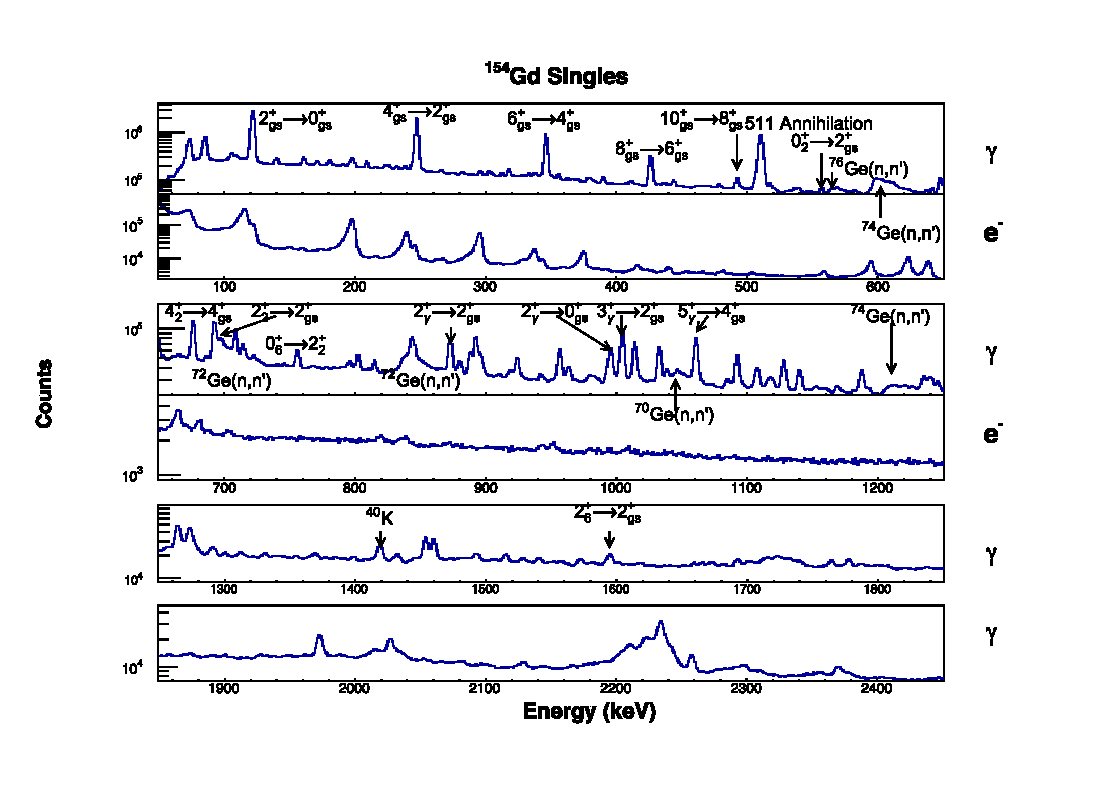
\includegraphics[scale=0.9]{154GdTablesAndFigs/154Gd_Singles_Label.eps}
    \caption[Singles spectra of $^{154}$Gd]{Singles spectra of $^{154}$Gd. Spectra are labeled with the particles being detected, the energies of the $\gamma$ and electron spectra aligned for identification. In the $\gamma$ spectrum, several lines of note are labeled. These are the ground-state band lines. In the conversion electron spectrum, the large peaks up to approximately 450 keV are from the ground state band. These large peaks make the ground state band a good diagnostic, but also emphasize the need for coincidence gating, as the conversion electron spectrum is flooded by the ground state band electrons. The large peak at low energy is cut off due to the threshold. It is a combination of background and the 123K peak. Transitions in the higher energy regime of the $\gamma$ spectrum cannot be determined without gating, due to additional background from the experimental room.}
    \label{fig:154Gd_Singles}
\end{figure}

These transitions in the ground state are the first lines looked at in the data. These lines are all pure E2 multipole transitions, making them an excellent diagnostic to compare with theoretical conversion coefficients. The transitions up to the $10^+$ are summarized and compared with theory in Table \ref{tab:154Gd_Single_ICC_GS}.

\afterpage{\clearpage\begin{landscape}
    \begin{longtable}{c|c|c|c|c|c|c|c|c|c|c}
        \caption{$^{154}$Gd Ground State Band Internal Conversion Coefficients from Singles}
        \label{tab:154Gd_Single_ICC_GS}\\
        \toprule
        $E$ (keV)	&	$J^{\pi}	\rightarrow	J^{\pi}$	&	$E_i$ (keV)	&	$E_f$ (keV)	&	$T_{1/2}$ (fs)	&	Multipolarity & Shell &	$\alpha$ (This Work)				&	$\alpha$  (Th)	&	$\alpha$ (Spits) & $\alpha$ (Gono)		\\
        \hline
        \endfirsthead
        \caption[]{$^{154}$Gd Ground State Band Internal Conversion Coefficients from Singles}\\
        \toprule
        $E$ (keV)	&	$J^{\pi}	\rightarrow	J^{\pi}$	&	$E_i$ (keV)	&	$E_f$ (keV)	&	$T_{1/2}$ (fs)	&	Multipolarity	& Shell &	$\alpha$ (This Work)				&	$\alpha$  (Th)	&	$\alpha$ (Spits) & $\alpha$ (Gono)	\\
        \hline
	    \endhead
	    \hline
        122.23	&	$2^+	\rightarrow	0^+$	&	123.0709	&	0	&	1184000	&	E2	&	K &	0.7759 (34) $^{+148}_{-146}$	&	0.656 (10)	& 0.61 (3) &		\\
    	&				&		&			&		&	& L	&	0.3788 (26) $^{+81}_{-80}$	&	0.411 (6)	&	&	\\
	    &				&		&		&			&	& M	&	0.1323 (3) (29)	&	0.0963 (14)	&	&	\\
	    \hline
        247.85	&	$4^+	\rightarrow	2^+$	&	370.9998	&	123.0709	&	45600	&	E2	&	K &	0.1044	(2) $^{+31}_{-30}$	&	0.1000 (12)	&	0.080 (3)	& 0.0827 (119)\\
	    &				&		&		&		& &	L	&	0.0272	(1) (8)	&	0.0225 (4)	&		\\
	    &				&		&		&		& & M	&	0.0096	(1) (3)	&	0.00513 (8)	&		\\
	    \hline
        346.59$^\dagger$	&	$6^+	\rightarrow	4^+$	&	717.662	&	370.9998	&	8260	&	E2 & K &	0.0335	(1)$^{+11}_{-10}$	&	0.0304 (5)	&	0.029 (1) & 0.0306*	\\
	    &				&		&		&		&	& L	&	0.0087	(1) (3)	&	0.00662 (10)	&		\\
	    &				&		&		&		&	& M	&	0.0027	(1)	(1) &	0.001491 (21)	&		\\
	    \hline
        426.84$^\dagger$	&	$8^+	\rightarrow	6^+$	&	1144.44	&	717.662	&	2570	&	[E2] & K & 0.0180	(2) (5)	&	0.01716 (24)	&	& 0.0170 (22)	\\
    	&				&		&		&		&	& L	&	0.0030	(1) (1)	&	0.00332 (5)	&		\\
	    &				&		&		&		&  	& M	&	0.0008	(1)	(1) &	0.000741 (11)	&		\\
	    \hline
        493.171	&	$10^+	\rightarrow	8^+$	&	1637.05	&	1144.44	&	1110	&	E2	& K	&	0.0124	(4) (4)	&	0.01179 (17)	& &	0.0124 (21)	\\
	    &				&		&		&		&	& L	&	0.0067	(4) (2)	&	0.00213 (3)	&		\\
        \bottomrule
    \end{longtable}
    \item{A list of ground state band conversion coefficients from $^{154}$Gd. Multipolarities and mixing ratios were taken from NNDC. Unless otherwise stated, the $\alpha$ values are $\alpha_K$. An angular distribution correction has been applied based on multipolarities for pure transitions, and those with known mixing ratios. The first error is statistical, the second is systematic. Numbers are compared with Spits et al.\citep{spits96:_154gd} and Gono et al.\citep{gono74:_154gd_e0} The starred value was used as an absolute calibration of the conversion electron detector in the Gono work. The dagger lines had contaminant lines subtracted from the conversion electrons. See the text for more details.}
\end{landscape}}

For the $6^+\rightarrow 4^+$ and $8^+\rightarrow 6^+$ transitions, electron contributions from smaller gamma lines of similar energy had to be subtracted. This was determined by looking at the conversion coefficients of these transitions in gated spectra, as discussed in the next section. Looking at Figure \ref{fig:154Gd_Singles}, it is clear there are many transitions around the same energy, so the contributions may be many. However, only lines from reactions in the target material will contribute. Gating isolates and identifies these lines for removal.

In the gated spectra, the internal conversion coefficients were in agreement with theory, meaning the transitions did not have contaminants when gated. In the singles, to remove the contaminant the gamma-ray had been seen and identified with known multipolarity. The conversion coefficient was then assumed from theory, and the contribution to the area was calculated to be

\begin{equation}
    \label{eq:ICC_Subtract}
    A_{e} = \alpha \epsilon_{e} \frac{A_{\gamma}}{\epsilon_{\gamma}} C_{\angle}
\end{equation}

where $\epsilon_{i}$ are the efficiencies of the electrons and gammas respectively. $C_{\angle}$ is the angular correction for this particular transition, discussed in Chapter \ref{chap:theory}. Here, it is multiplied, and not divided, so it can be subtracted from the uncorrected area.

The calculated contributions were subtracted off the fitted area of the electron peak, before the conversion coefficient was calculated. This meant the error also include contributions from the errors of these gamma peaks and the errors on the theoretical $\alpha$ values. 

There were two types of transitions that acted as contaminants: those of similar energy, and higher energies whose K-electron energies were similar to the L and M peaks of the lines of interest. The peaks are summarized in Table \ref{tab:154Gd_Contaminants}. The electron-shell of the contaminant is listed in each case, and total $L$ and $M$ contributions are used, without need to look at subshell contributions.  In the case of several contaminant transitions, the mixing ratio had to be assumed to get a conversion coefficient for the subtraction.

\afterpage{\clearpage\begin{table}[!]
    \centering
    \begin{longtable}{>{\small}c|>{\small}c|>{\small}c|>{\small}c|>{\small}c|>{\small}c|>{\small}c|>{\small}c}
        \caption{$^{154}$Gd Ground State Band $6^+\rightarrow 4^+$ and $8^+\rightarrow 6^+$ Extra Electron Peak Contributions in Singles}
        \label{tab:154Gd_Contaminants} \\
        \toprule
         $E$ & $E_i$ & $E_f$ & $J_i\rightarrow J_f$ & Multipolarity & $\delta$ & Shell & $\alpha$  \\ \hline
         \endhead
         \endfoot
         \endlastfoot
         \multicolumn{8}{l}{346.59 keV, $6^+\rightarrow 4^+$} \\ \hline
         338.28 & 1770 & 1432 & $5^+_{4^+}\rightarrow 5^+_{\gamma}$ & E0,E2,M1 & -0.004 & K & 0.10 (1) \\ 
         & & & & & $\frac{K(E0)}{K(E2)}\approx 1.0$ & L & 0.01210 (12) \\ 
         & & & & & & M & 0.00180 (3) \\ \hline
         342.18 & 2254 & 1911 & $8^+_{4^+}\rightarrow 6^+_{4^+}$ & E2 & & K & 0.0315 (5) \\ 
         & & & & & & L & 0.0069 (1) \\\
         & & & & & & M & 0.001554 (22) \\ \hline
         390.73 & 1756 & 1366 & $8^+_{0^+_2}\rightarrow 6^+_{0^+_2}$ & E2 & & K & 0.0218 (3) \\ \hline
         \multicolumn{8}{l}{426.84 keV, $8^+\rightarrow 6^+$} \\ \hline
         422.12 & 1418 & 996 & $2^+_{0^+_3}\rightarrow 2^+_{\gamma}$ & E0,E2,M1 & Assumed $\approx 1$ & K & 0.114 (16) \\ 
         & & & & & & L & 0.0161 (23) \\ 
         & & & & & & M & 0.0049 (12) \\ \hline
         466.99 & 1719 & 1251 & $2^-_{2^-}\rightarrow 3^-_{0^-}$ & M1,E2 & Assumed $\approx 1$ & K & 0.019 (6) \\ \hline
         478.27 & 1719 & 1241 & $2^-_{2^-}\rightarrow 1^-_{0^-}$ & E2 & & K & 0.01272 (18) \\
         \bottomrule
         \multicolumn{8}{p{\textwidth}}{Table \ref{tab:154Gd_Contaminants}: A list of the transitions in the $^{154}$Gd Singles data that were contributing to the electron peaks corresponding to the ground state band lines. Conversion coefficients were assumed using BrICC\citep{kibedi08:_BRICC}. The bands for each level are listed as subscripts.}
    \end{longtable}
\end{table}}

\section{Gates on the Ground State Band}
\label{sec:154GS_Gates}

The transitions of the ground state band were the most prominent seen in the gamma-ray and conversion electron spectra, as seen in Figure \ref{fig:154Gd_Singles}. To build a level scheme based on known levels and transitions, the $\gamma$ components of these transitions were gated on. Figures \ref{fig:154_2to0level}, \ref{fig:154_4to2}, \ref{fig:154_6to4}, and \ref{fig:154_8to6} are the result of these gates. Band structure in these figures was taken from the data sheets. No band assignments were made in this work. In the cases of cascades, secondary gates were done to confirm assignments.

Determining which transitions went uniquely into a given ground state level was done by comparing the outgoing ground state transition for that level with the incoming transition i.e. for the $2^+$ level, the $2^+\rightarrow0^+$ (123 keV) gate was compared directly with the $4^+\rightarrow2^+$ (247 keV) gate. The $\gamma$-spectra corresponding to these gates can be seen in Figure \ref{fig:154_GS_Gate}. Lines in the gamma spectrum that were present only in the outgoing spectrum, but not the incoming, were assumed to be populating that level (the $2^+$ state in the above example). These identified transitions were then gated on for two reasons: to confirm where the line populated the ground-state band, and to search for cascades from higher states.

\begin{landscape}
\begin{figurels}[!]
    \caption{\fontsize{10pt}{12pt} Spectra gated on 123 keV ($2_{gs}^+\rightarrow 0_{gs}^+$) and 247 keV ($4_{gs}^+\rightarrow 2_{gs}^+$), the first two ground state band lines of $^{154}$Gd. As can be seen, some lines do not appear in different gates. Comparison of these gates, yields a list of transitions that directly populate the interim level (in this example, the $2^+$ state). Several peaks are circled in green that appear in the $2_{gs}^+\rightarrow 0_{gs}^+$ and not the $4_{gs}^+\rightarrow 2_{gs}^+$ transition.}
    \label{fig:154_GS_Gate}
\end{figurels}
\begin{figurels}[!]
    \centering
    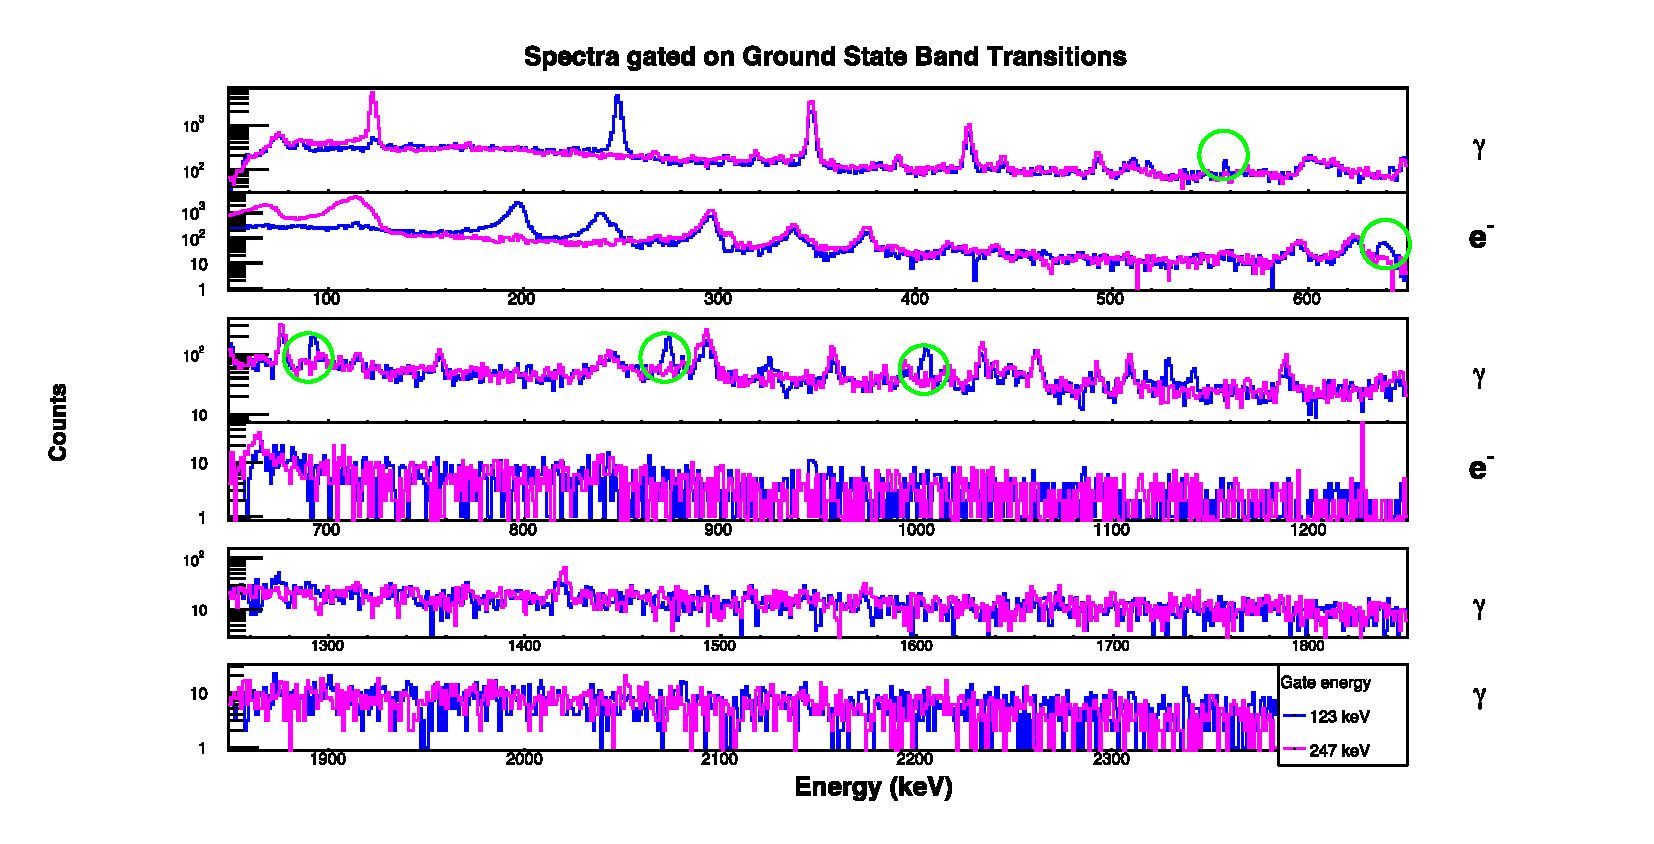
\includegraphics[scale=0.9]{154GdTablesAndFigs/154Gd_stacked.eps}
\end{figurels}
\end{landscape}

There were nine bands seen in the gating outside of the ground state band, 4 of which are bands with excited $0^+$ band heads. These are seen in the $2^+\rightarrow0^+$ gate (Figure \ref{fig:154_2to0}). Three of these bands are seen in the $4^+\rightarrow2^+$ gate (Figure \ref{fig:154_4to2}), and two are seen in the $6^+\rightarrow4^+$ gate (Figure \ref{fig:154_6to4}). Only one is seen in the $8^+\rightarrow6^+$ gate (Figure \ref{fig:154_8to6}). This drop off is not surprising due to the lack of known higher spin states in the higher energy $0^+$ bands. Additionally, there is a drop off in populating higher energy states in the nucleus.

\begin{landscape}
\begin{figure}[!]
    \centering
    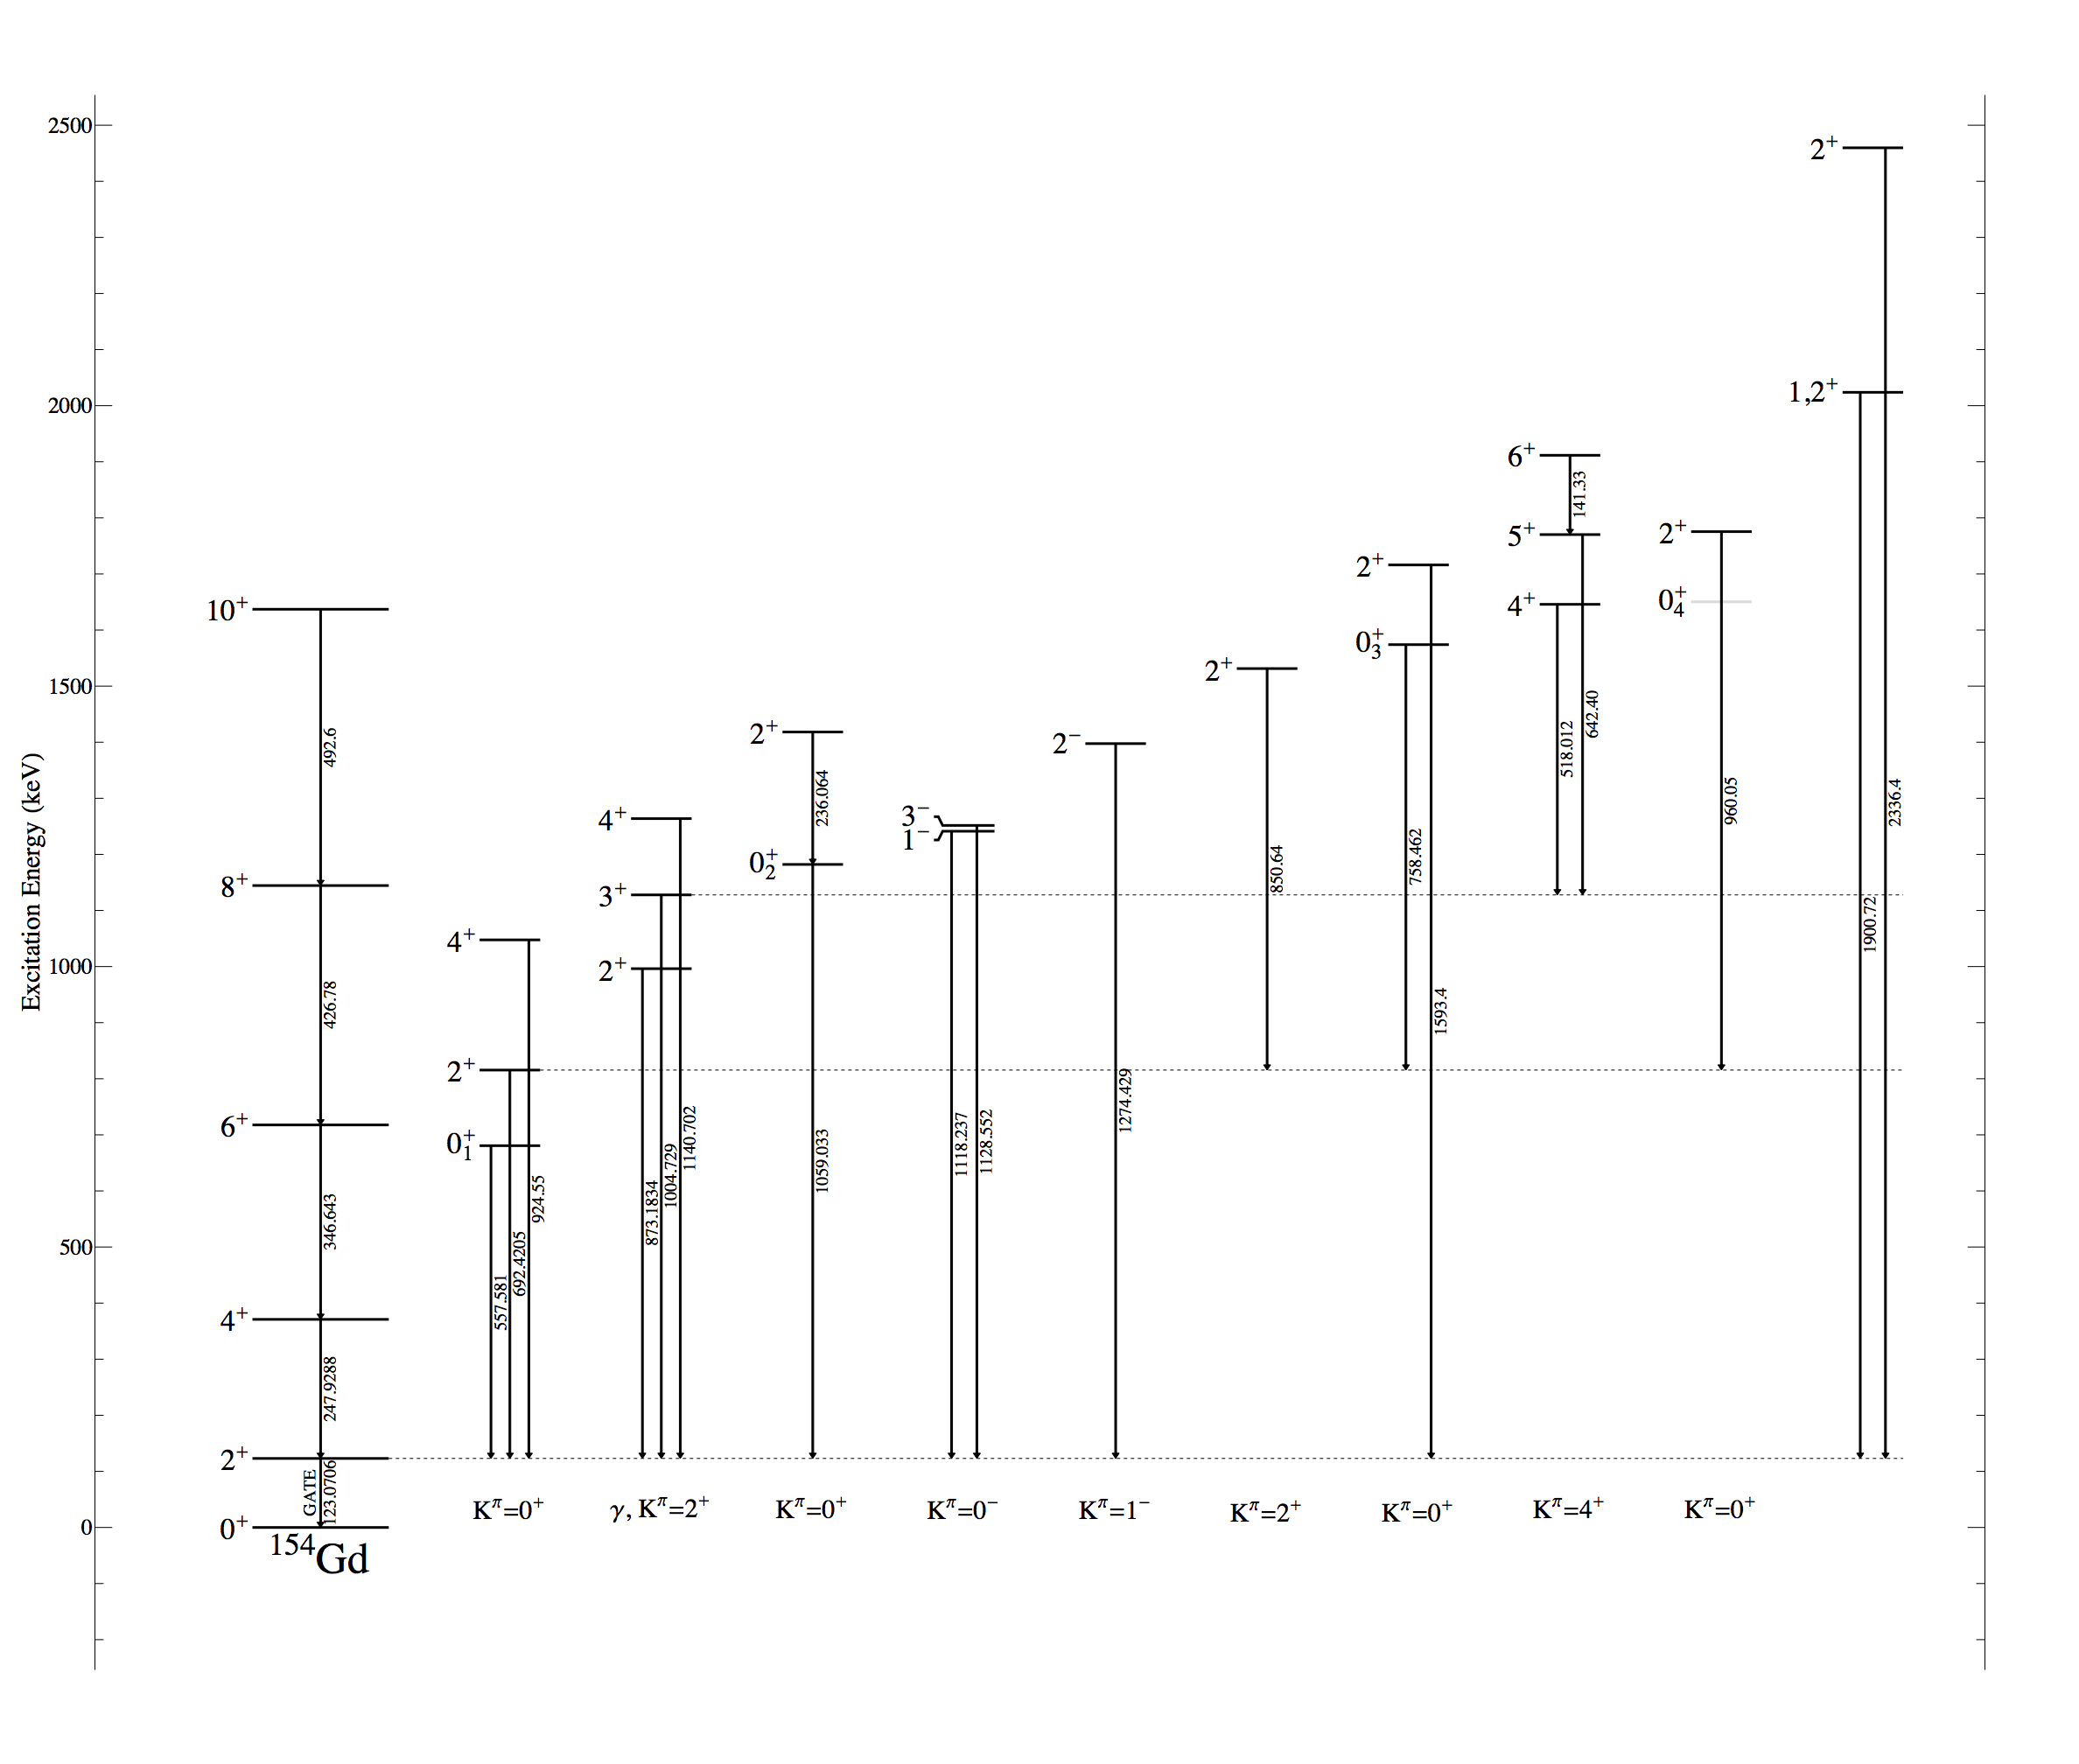
\includegraphics[scale=0.33]{154GdTablesAndFigs/154Gd_2to0.eps}
    \caption{Level Scheme of $^{154}$Gd. The gamma ray of the $2^+\rightarrow0^+$ transition (123 keV) in the ground state was gated on. It was then compared with the gated spectrum from the gamma ray of the $4^+\rightarrow2^+$ transition (247 keV) in the ground state. Peaks only appearing in the first gate and not higher energy gates were assumed to go into the $2^+$ state, and assignments were made. Due to the low energy of the $2^+\rightarrow0^+$ transition, the efficiency was lower, and it is likely that transitions into the $2^+$ state were missed. The levels are organized by band. The lower levels of the band, unseen by gamma rays in this gate, are in gray.}
    \label{fig:154_2to0}
\end{figure}
\end{landscape}

\begin{landscape}
\begin{figure}[!]
    \centering
    \captionlistentry{(a) Level Scheme of $^{154}$Gd. The gate on the $4_{gs}^+\rightarrow 2_{gs}^+$ transition (247 keV) $\gamma$-component in the ground state. The lines shown are in coincidence. The levels are organized by band. The lower levels of the band, unseen by gamma rays in this gate, are in blue. (b) Gamma spectrum gated on 247 keV, corresponding to the $4_{gs}^+\rightarrow 2_{gs}^+$ transition. Several transitions have been labeled, corresponding to the level scheme.}
    \label{fig:154_4to2}
    \begin{subfigure}{1.4\textwidth}
    \caption{\centering \fontsize{10pt}{12pt}Level Scheme of $^{154}$Gd. The gate on the $4_{gs}^+\rightarrow 2_{gs}^+$ transition (247 keV) $\gamma$-component in the ground state. The lines shown are in coincidence. The levels are organized by band. The lower levels of the band, unseen by gamma rays in this gate, are in blue. (b) Gamma spectrum gated on 247 keV, corresponding to the $4_{gs}^+\rightarrow 2_{gs}^+$ transition. Several transitions have been labeled, corresponding to the level scheme.}
    \end{subfigure}
\end{figure}
\clearpage
\begin{figure}
    \ContinuedFloat
    \begin{subfigure}{1.4\textwidth}
    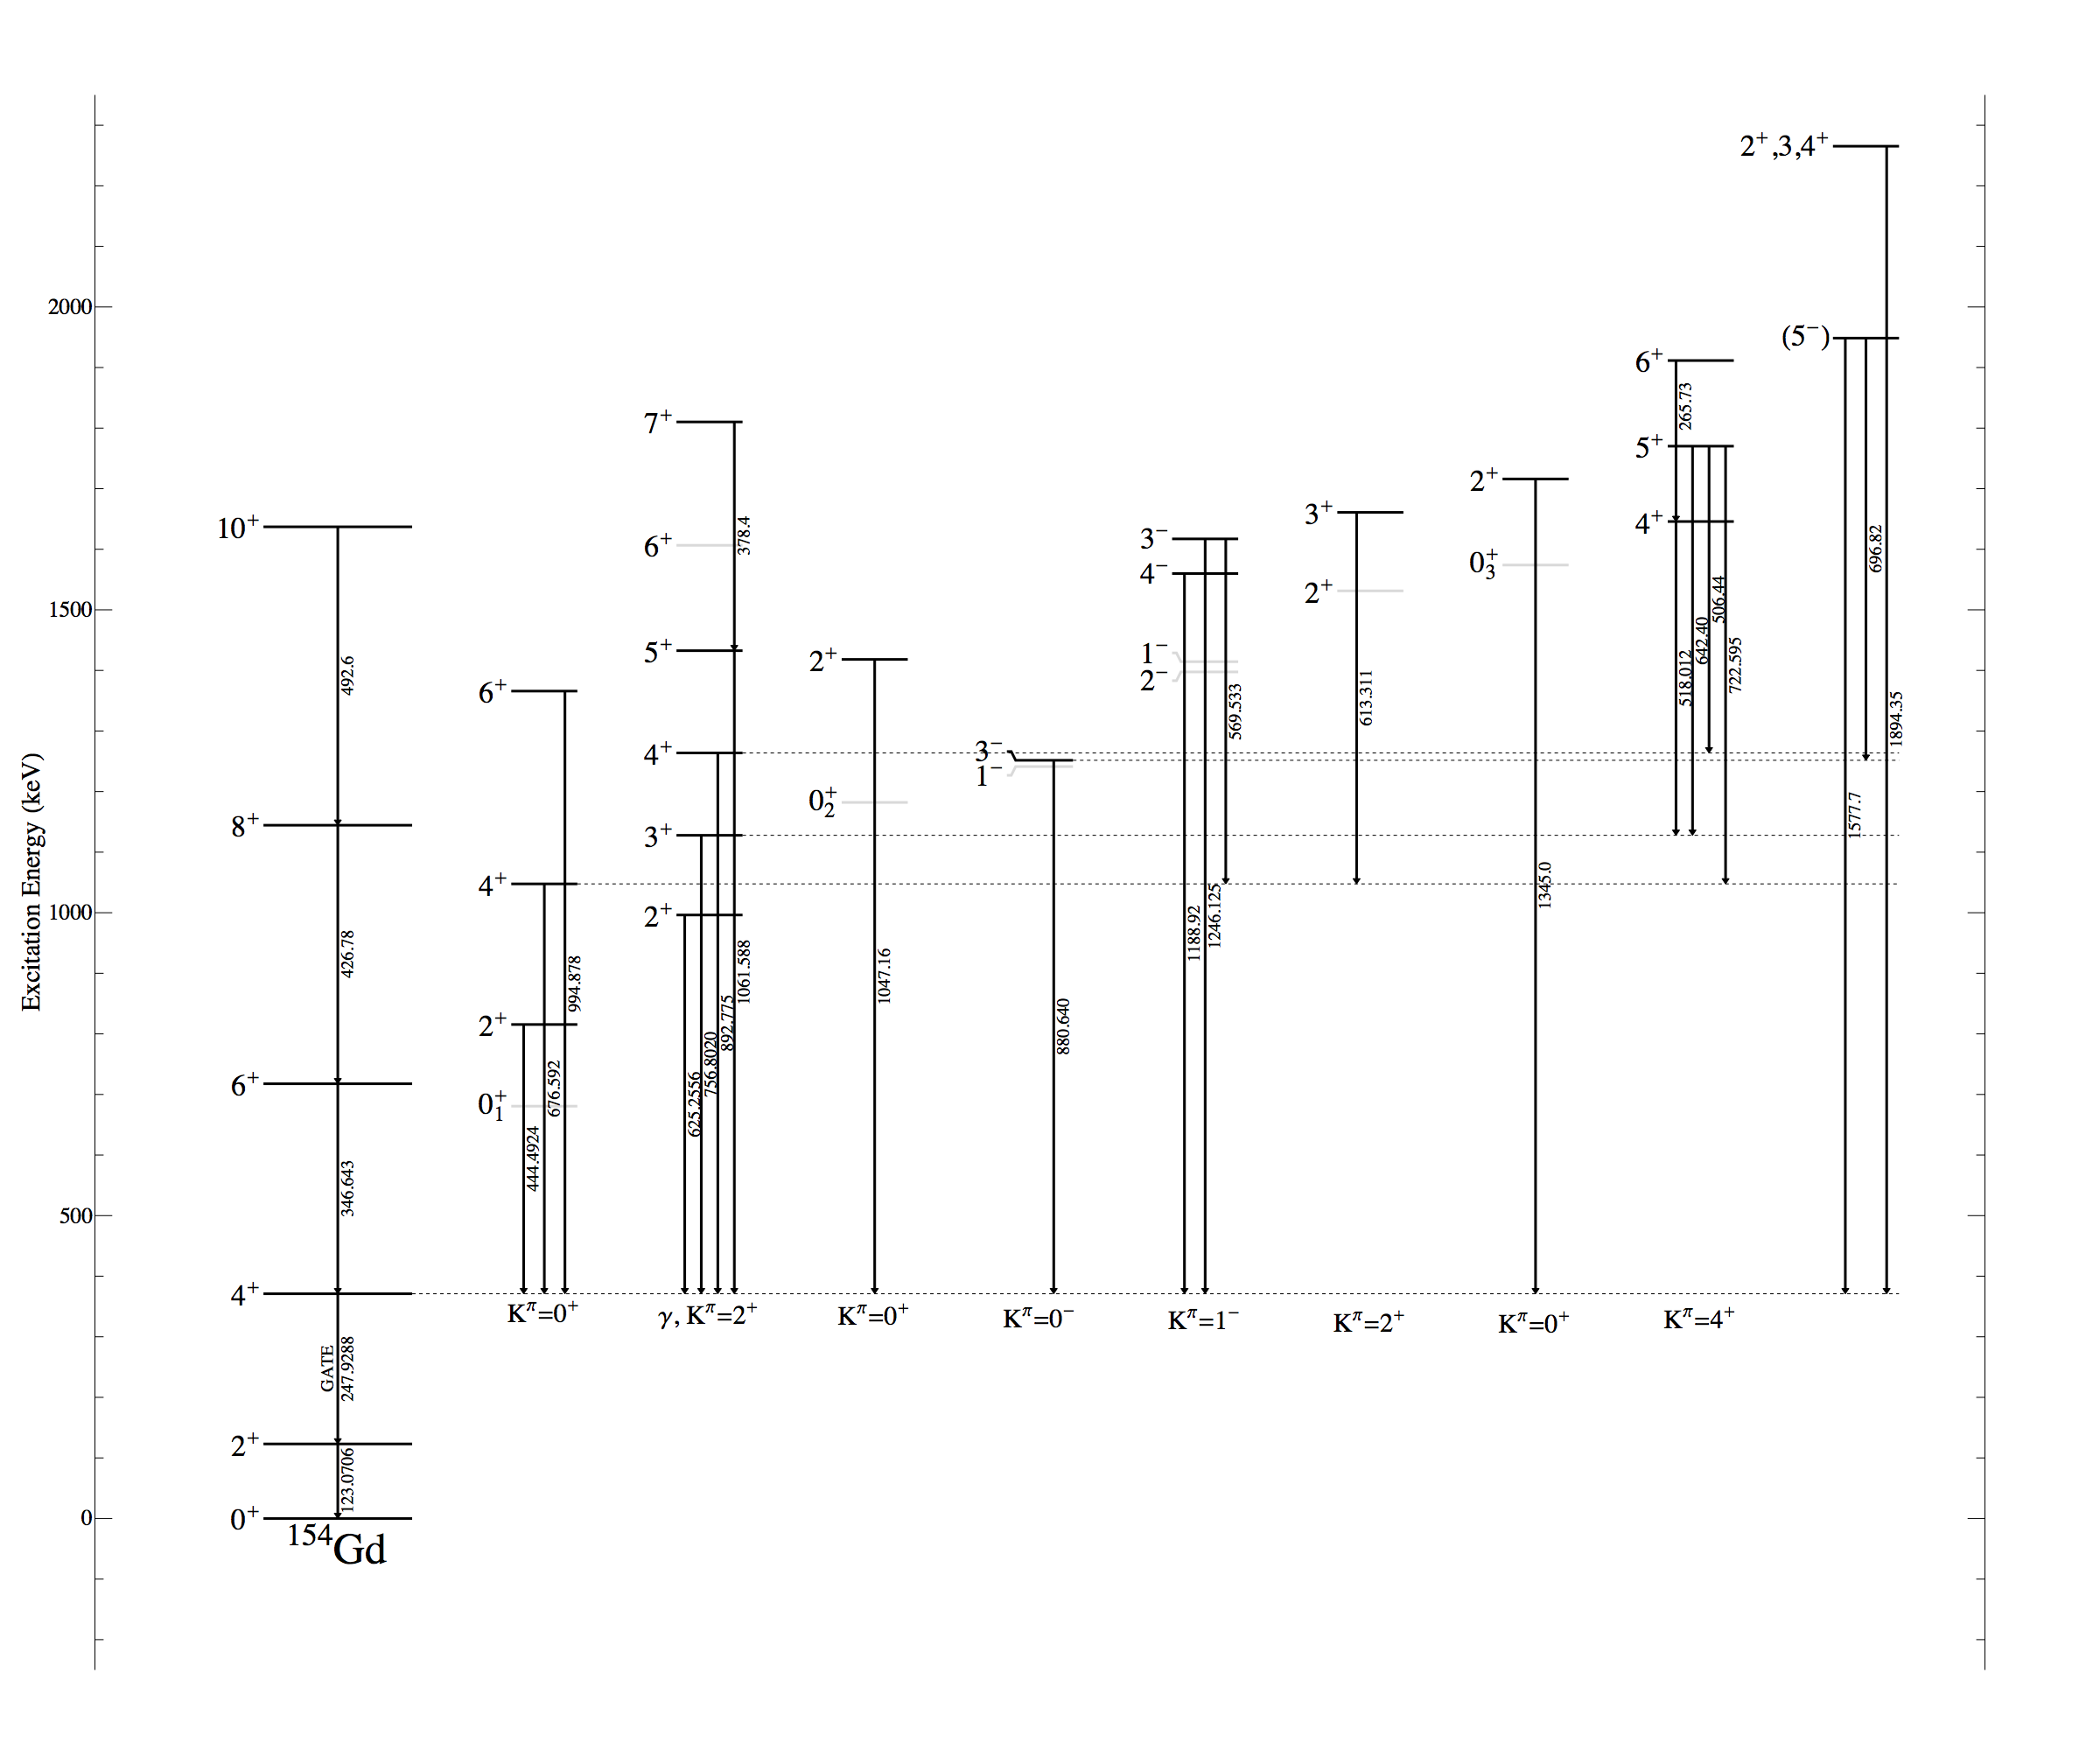
\includegraphics[scale=0.33]{154GdTablesAndFigs/154Gd_4to2.eps}
    \caption*{(a)}
    \label{fig:154_4to2level}
    \end{subfigure}
    \end{figure}
    \end{landscape}
    \begin{figure}
    \ContinuedFloat
    \begin{subfigure}{\textwidth}
    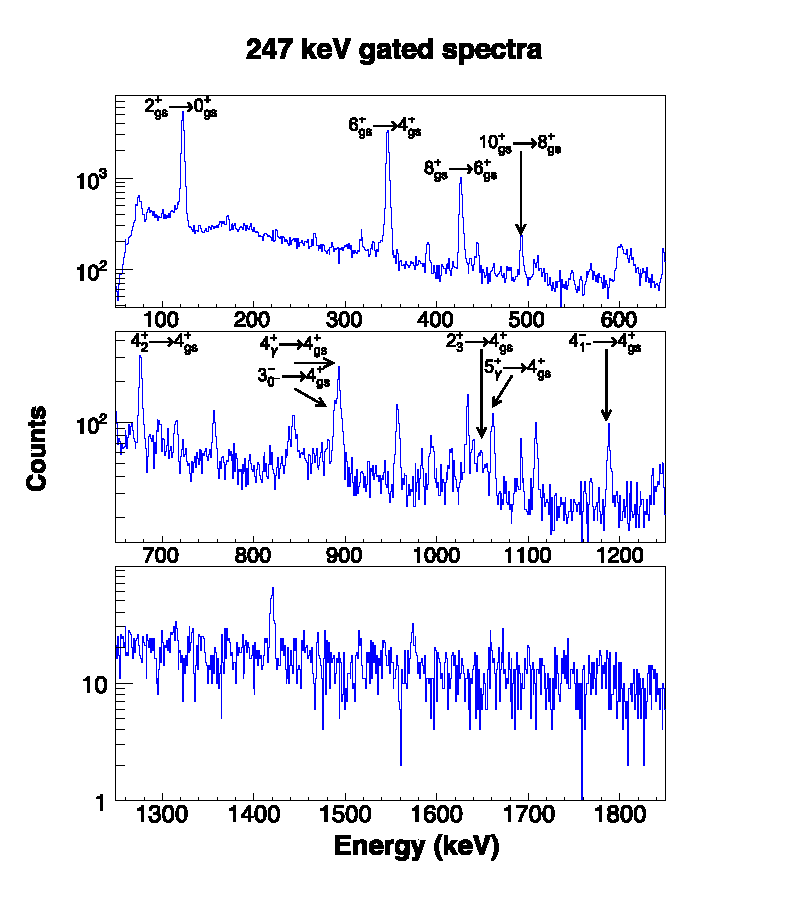
\includegraphics[scale=1.3]{154GdTablesAndFigs/247_gamma.eps}
    \caption*{(b)}
    \label{fig:154_4to2spec}
    \end{subfigure}
\end{figure}

\begin{landscape}
\begin{figure}[!]
    \centering
    \captionlistentry{(a) Level Scheme of $^{154}$Gd. The gate on the $6_{gs}^+\rightarrow 4_{gs}^+$ transition (346 keV) $\gamma$-component in the ground state. The lines shown are in coincidence. The levels are organized by band. The lower levels of the band, unseen by gamma rays in this gate, are in blue. (b) Gamma spectrum gated on 346 keV, corresponding to the $6_{gs}^+\rightarrow 4_{gs}^+$ transition. Several transitions have been labeled, corresponding to the level scheme.}
    \label{fig:154_6to4}
    \begin{subfigure}{1.4\textwidth}
    \caption{\centering \fontsize{10pt}{12pt}Level Scheme of $^{154}$Gd. The gate on the $6_{gs}^+\rightarrow 4_{gs}^+$ transition (346 keV) $\gamma$-component in the ground state. The lines shown are in coincidence. The levels are organized by band. The lower levels of the band, unseen by gamma rays in this gate, are in blue. (b) Gamma spectrum gated on 346 keV, corresponding to the $6_{gs}^+\rightarrow 4_{gs}^+$ transition. Several transitions have been labeled, corresponding to the level scheme.}
    \end{subfigure}
\end{figure}
\clearpage
\begin{figure}
    \ContinuedFloat
    \begin{subfigure}{1.4\textwidth}
    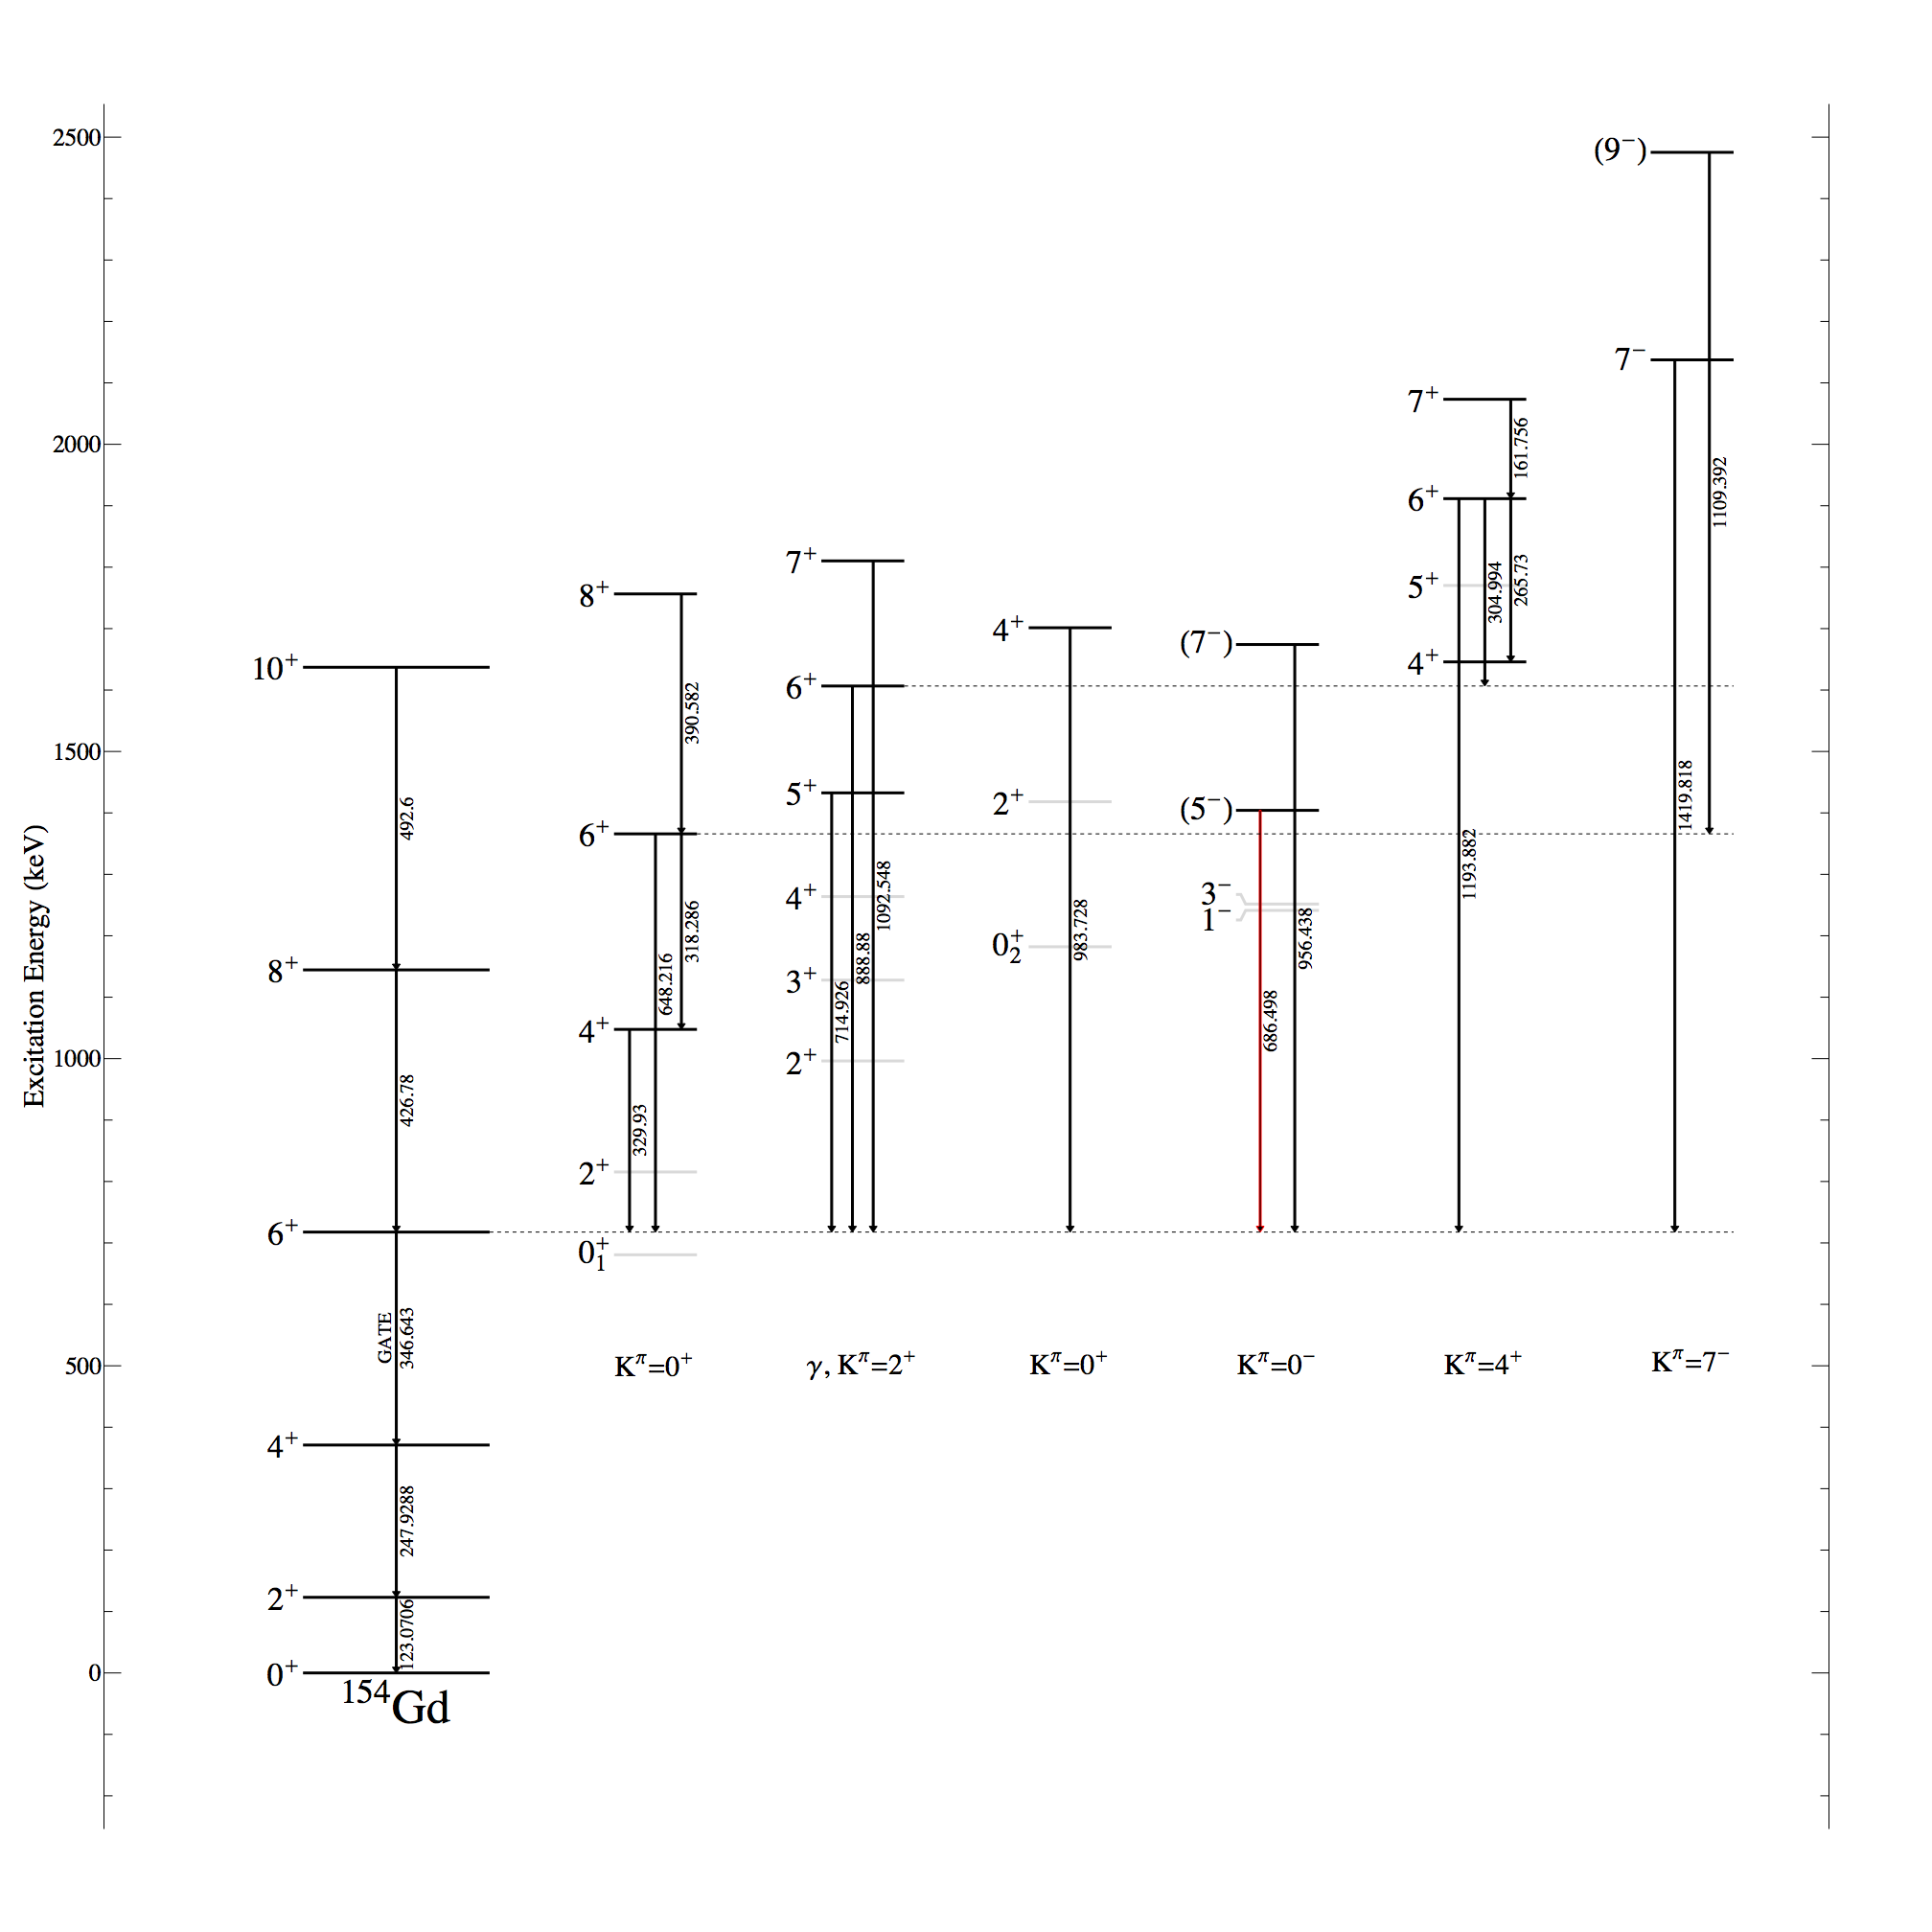
\includegraphics[scale=0.33]{154GdTablesAndFigs/154Gd_6to4.eps}
    \caption*{(a)}
    \end{subfigure}
    \end{figure}
    \end{landscape}
    \begin{figure}
    \ContinuedFloat
    \begin{subfigure}{\textwidth}
    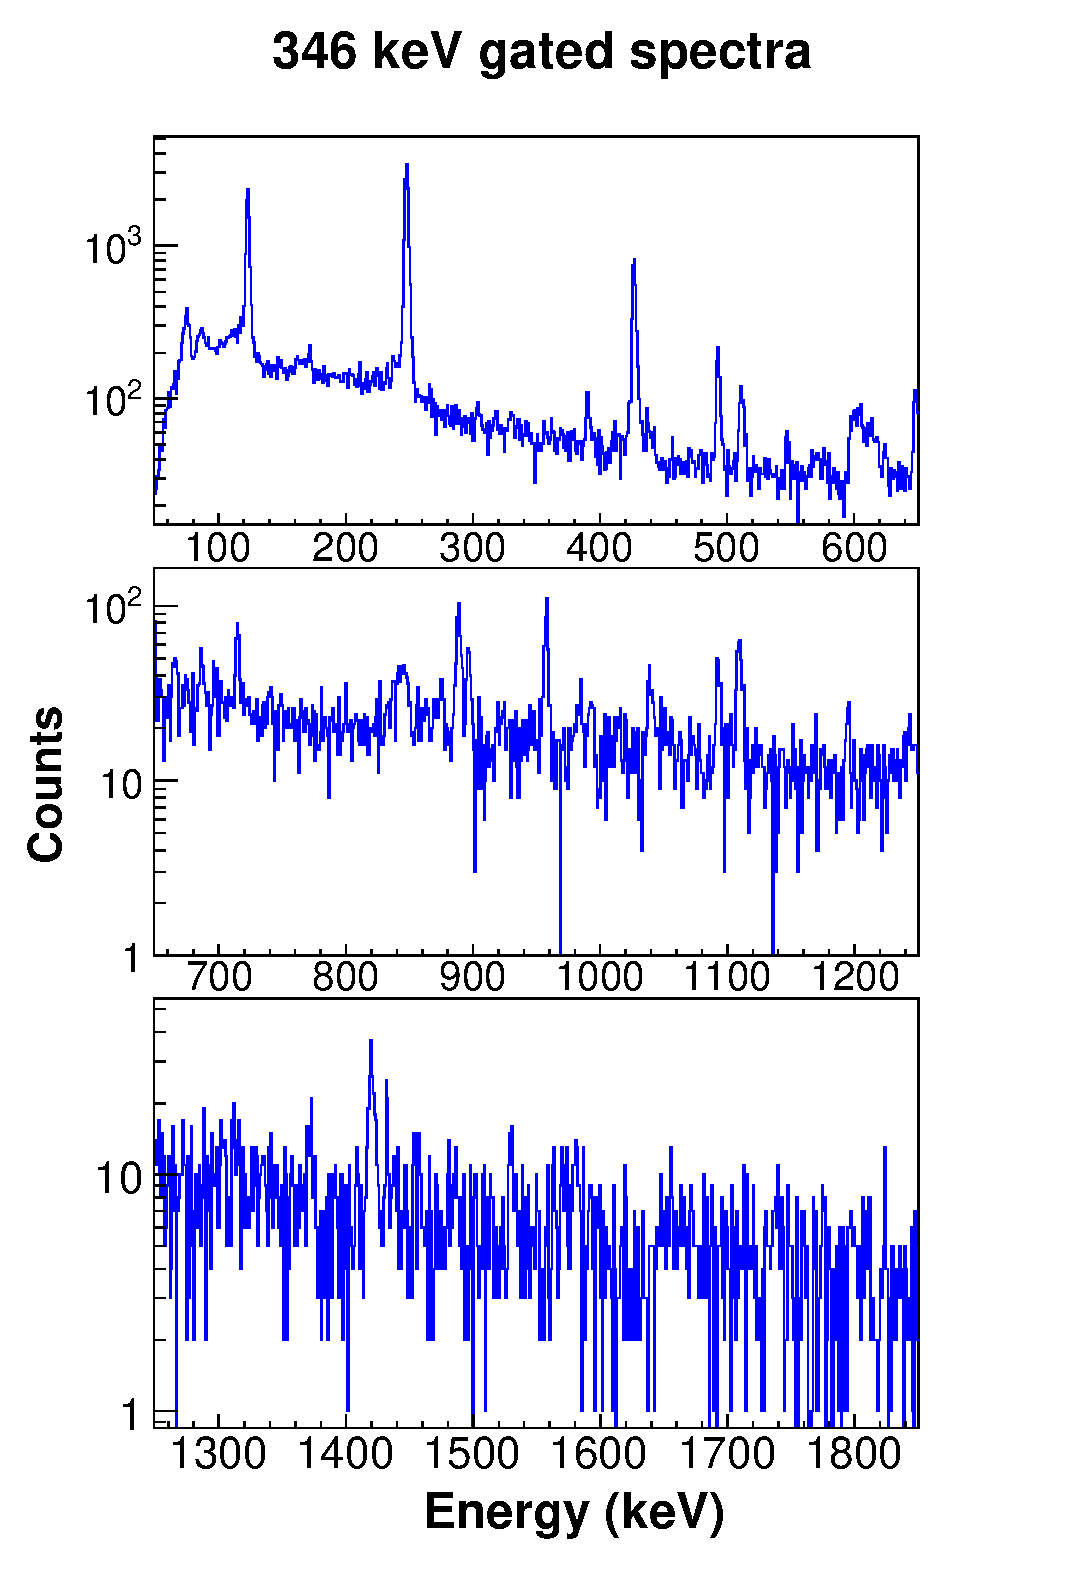
\includegraphics[scale=1.3]{154GdTablesAndFigs/346_gamma.eps}
    \caption*{(b)}
    \label{fig:154_6to4spec}
    \end{subfigure}
\end{figure}

\begin{figure}[!]
    \centering
    \begin{subfigure}{\textwidth}
    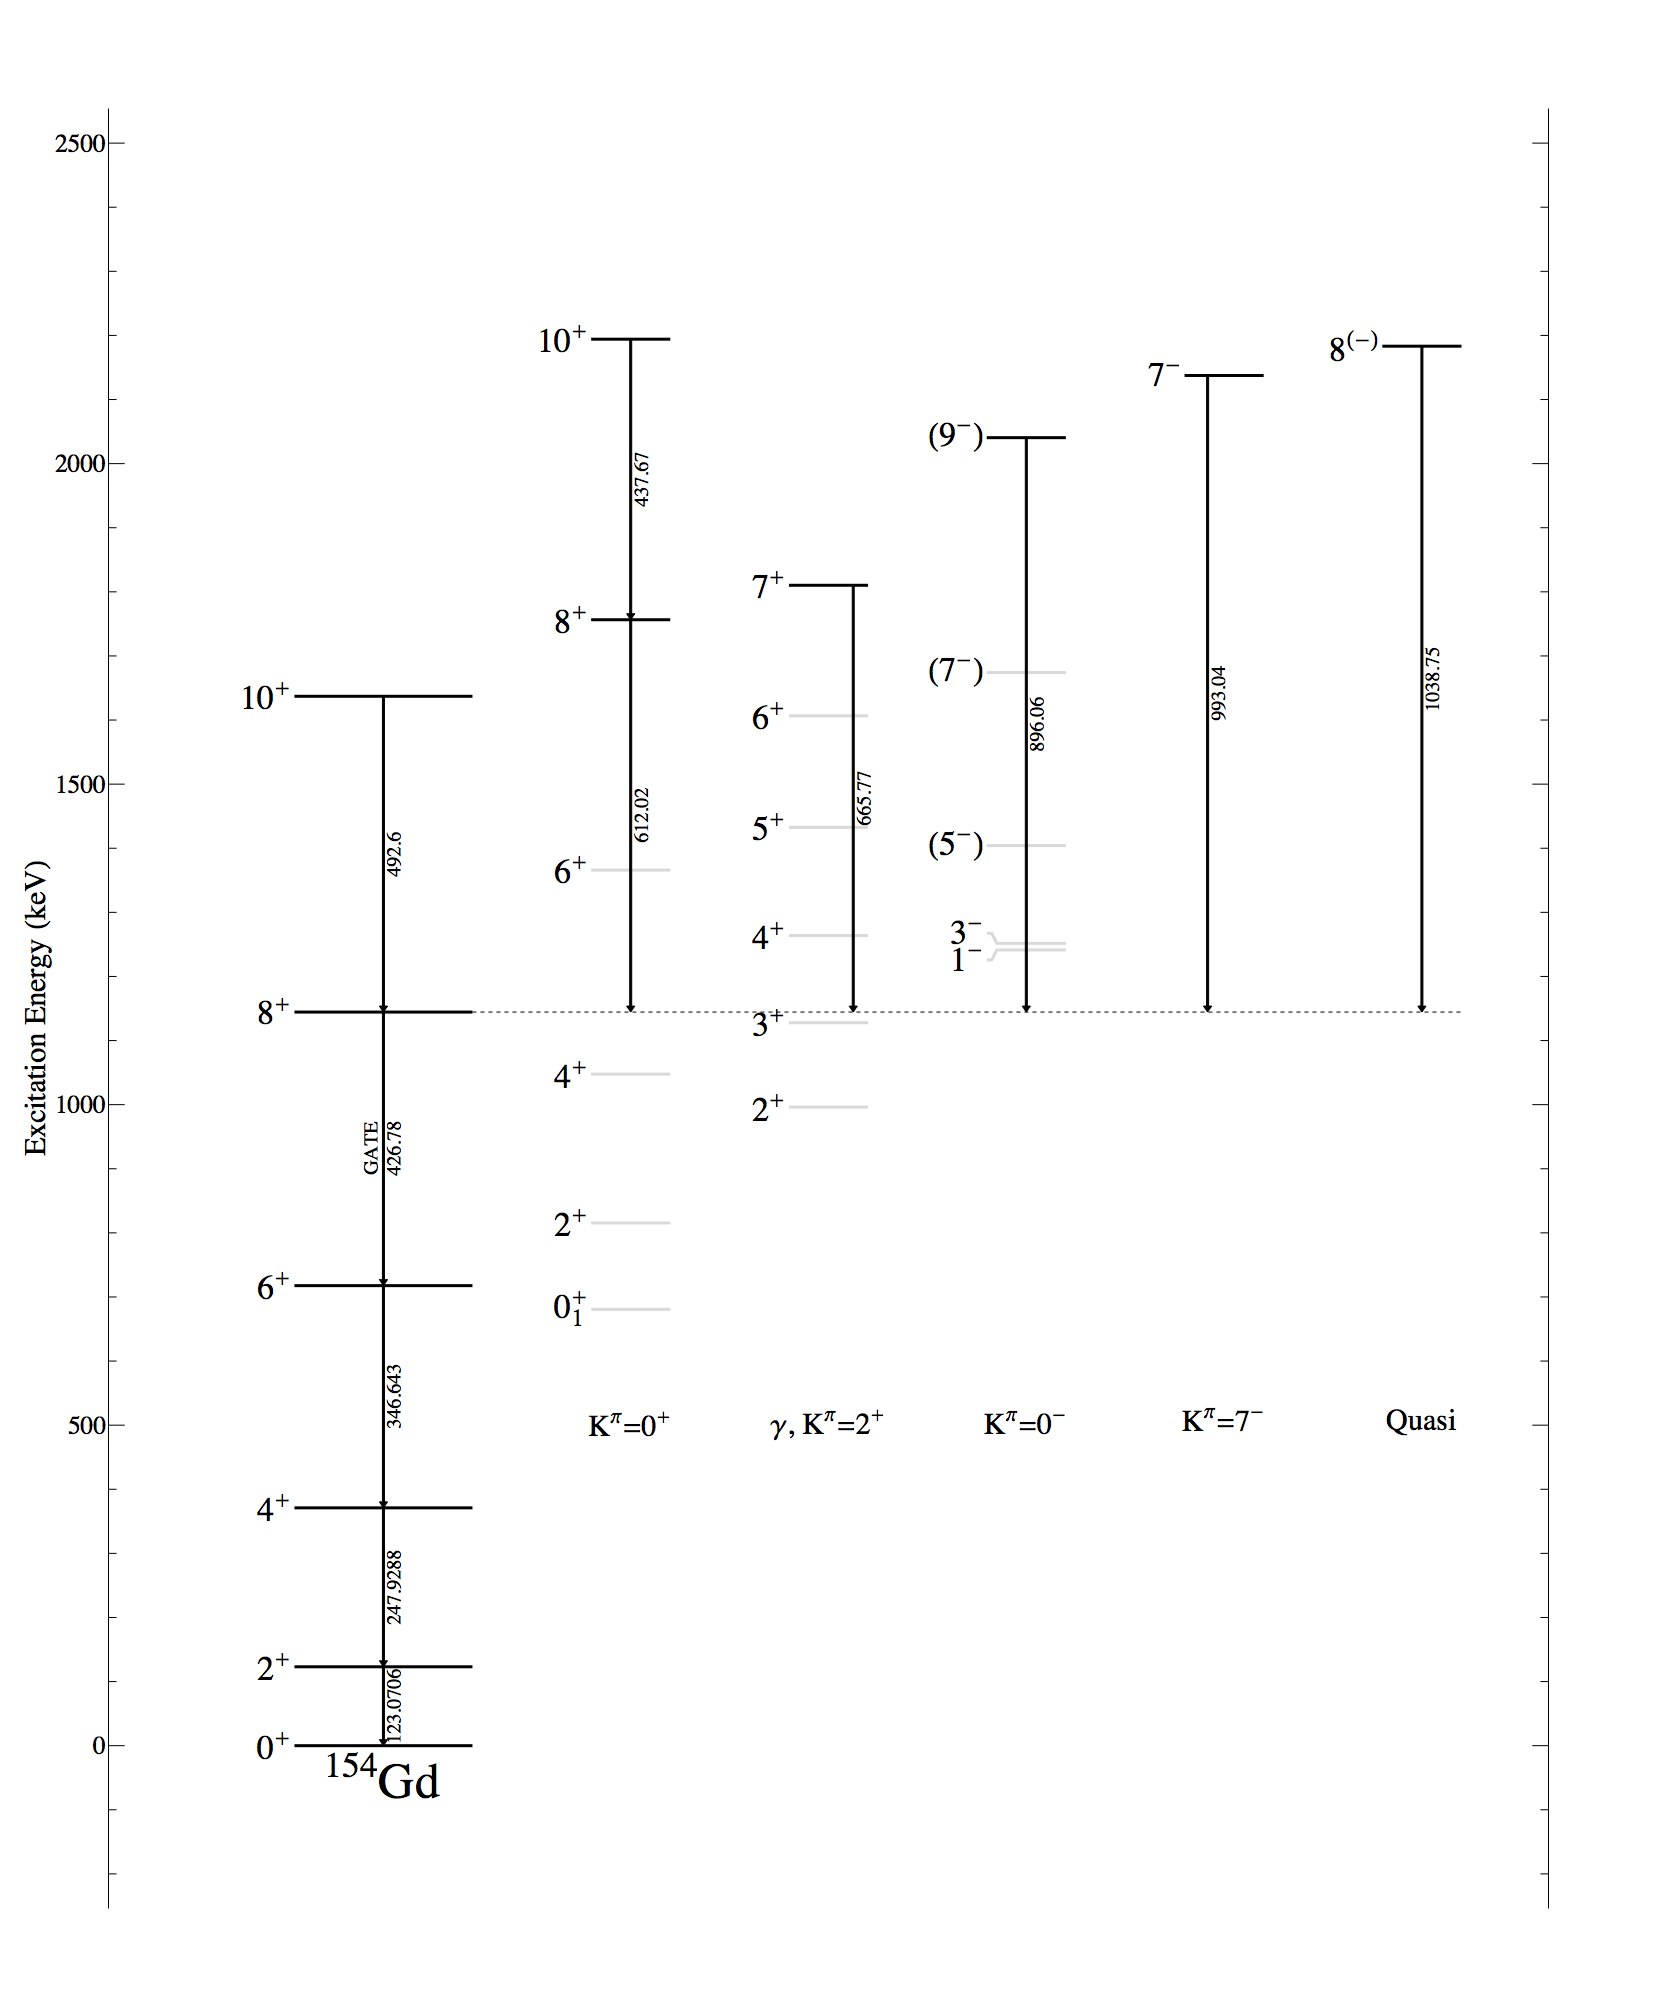
\includegraphics[scale=0.33]{154GdTablesAndFigs/154Gd_8to6.eps}
    \caption{\label{fig:154_8to6level}Level Scheme of $^{154}$Gd. The gamma ray of the $8^+\rightarrow6^+$ transition (426 keV) in the ground state was gated on. It was then compared with the gated spectrum from the gamma ray of the $10^+\rightarrow8^+$ transition (492 keV) in the ground state. Peaks only appearing in the first gate were assumed to go into the $8^+$ state, and assignments were made. Additionally, these peaks were also gated on, to look for cascades leading into the $8^+$ state, which were found in several cases. The levels are organized by band. The lower levels of the band, unseen by gamma rays in this gate, are in gray.}
    \end{subfigure}
    \captionlistentry{Level scheme and spectrum of $^{154}$Gd based on the $8^+\rightarrow6^+$ transition.}
    \label{fig:154_8to6}
    \end{figure}
    \begin{figure}
    \ContinuedFloat
    \begin{subfigure}{\textwidth}
    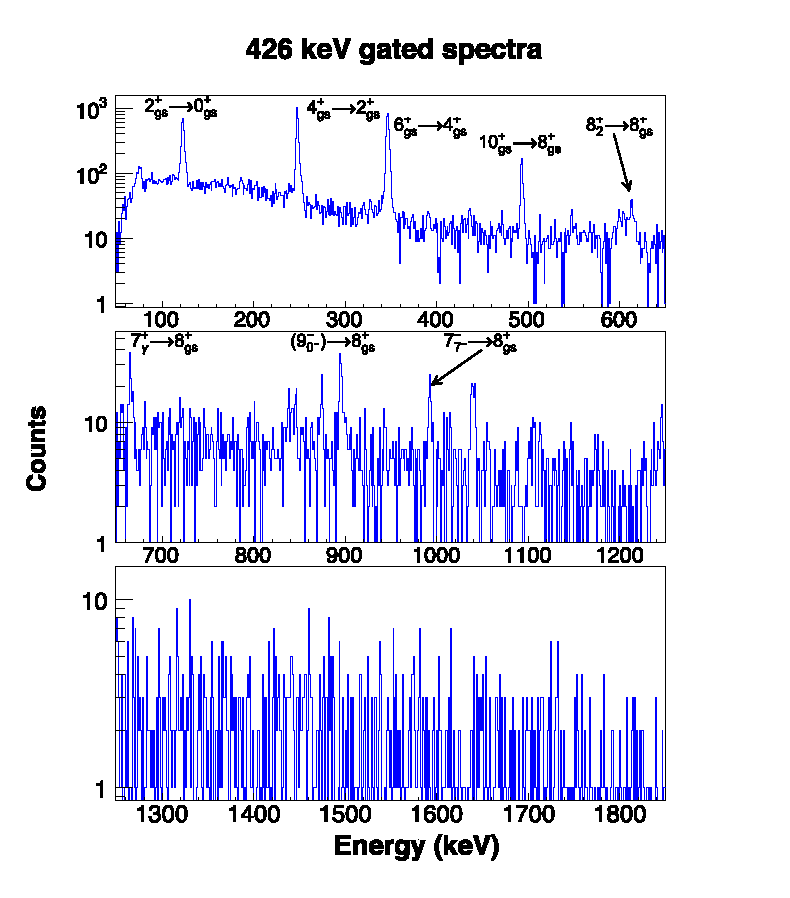
\includegraphics[scale=0.8]{154GdTablesAndFigs/426_gamma.eps}
    \caption{Gamma spectrum gated on 426 keV, corresponding to the $8^+\rightarrow6^+$ transition.}
    \label{fig:154_6to4spec}
    \end{subfigure}
\end{figure}

\section{Conversion Coefficients from Singles}
\label{sec:154_Conv_Singles}

With the gamma-rays now identified through gates, conversion coefficients could be calculated from the singles spectra. Transitions that could be clearly identified and separated are found in Table \ref{tab:154Gd_Single_ICC}. Contamination concerns were taken into account by using the identified transitions to look for gamma-rays in close proximity to those in the Table. Several transitions with E0 components can be found in the table. Most of the conversion electrons seen are the $K$-shell electron. These transitions could be given an angular correction based on the multipolarity of the transition.

Table \ref{tab:154Gd_Single_ICC_Uncorr} holds conversion coefficients that have been left uncorrected in the singles for one of two reasons: either there were multiple known assignments to the gamma-ray energy, or the exact multipole mixing-ratio was unknown. Table \ref{tab:154Gd_No_Mult_ICC} contains the conversion coefficients that could not be corrected because the transition has no multipole assignment. It contains allowable and reasonable theoretical conversion coefficients to compare the values against, calculated using BrIcc \cite{kibedi08:_BRICC}.

\afterpage{\clearpage\begin{table}
    \centering
    \caption{$^{154}$Gd Internal Conversion Coefficients from Singles}
    \label{tab:154Gd_Single_ICC}
\begin{ThreePartTable}
    \begin{tabular}{c|c|c|c|c|c|c}
        \multicolumn{7}{>{\fontsize{12}{15}}c}{(a)}\\
        \toprule
        $E$ (keV)	&	$J^{\pi}	\rightarrow	J^{\pi}$	&	$E_i$ (keV)	&	$E_f$ (keV)	&	$T_{1/2}$ (fs)	&	Multipolarity	&	$\delta$\\
        \hline
        232.44	&	$4^+_{0^+_2}	\rightarrow	2^+_{0^+_2}$	&	1047.592	&	815.4917	&	7600	&	E2	&	\\
	    &				&		&		&		&		& \\
	    \hline
        329.49	&	$4^+_{0^+_2}	\rightarrow	6^+_{gs}$	&	1047.592	&	717.662	&	7600	&	E2	&	\\
        \hline
        349.89	&	$2^+_{2^+_2}	\rightarrow	0^+_{gs}$	&	1531.305	&	1182.091	&		&	[E2]	&	 \\
        \hline
        416.79	&	$4^+_{0^+_6}	\rightarrow	3^+_{2^+_2}$	&	2080.23	&	1660.903	&		&	(M1)	&	\\
        \hline
        444.19	&	$2^+_{0^+_2}	\rightarrow	4^+_{\gamma}$	&	815.4917	&	370.9998	&	6400	&	E2	&		\\
        \hline
        506.41	&	$5^+_{4^+_1}	\rightarrow	4^+_{\gamma}$	&	1770.187	&	1263.778	&		&	E2	&		\\
        \hline
        515.92	&	$4^+_{4^+_1}	\rightarrow	3^+_{\gamma}$	&	1645.814	&	1127.802	&		&	E2+M1	&	-7 (3)	\\
        \hline
        557.58	&	$0^+_{0^+_2}	\rightarrow	2^+_{gs}$	&	680.6673	&	123.0709	&	4560	&	E2	&		\\
        \hline
        610.71	&	$8^+_{0^+_2}	\rightarrow	8^+_{gs}$	&	1756.49	&	1144.44	&		&	E0+M1+E2	&	-0.69 (14)	\\
	    &				&		&		&		&		&	\\
	    \hline
        676.70	&	$4^+_{0^+_2}	\rightarrow	4^+_{gs}$	&	1047.592	&	370.9998	&	7600	&	E0+M1+E2	&	+2.9 (4)	\\
        \hline
        693.47	&	$2^+_{0^+_2}	\rightarrow	2^+_{gs}$	&	815.4917	&	123.0709	&	6400	&	E2+M1+E0	&	7.5 (4)	\\
        \hline
        873.54	&	$2^+_{\gamma}	\rightarrow	2^+_{gs}$	&	996.2568	&	123.0709	&	950	&	E2+M1+E0	&	-9.4 (4)	\\
        \hline
        889.61	&	$6^+_{\gamma}	\rightarrow	6^+_{gs}$	&	1606.55	&	717.662	&		&	E2+M1	&	$>1.8$	\\
        \hline
        894.40	&	$4^+_{\gamma}	\rightarrow	4^+_{gs}$	&	1263.778	&	370.9998	&		&	E0+M1+E2	&	-3.8 (3)	\\
        \hline
        924.85	&	$4^+_{0^+_2}	\rightarrow	2^+_{gs}$	&	1047.592	&	123.0709	&	7600	&	E2	&	\\
        \hline
        996.33	&	$2^+_{\gamma}	\rightarrow	0^+_{gs}$	&	996.2568	&	0	&	950	&	E2	&	\\
        \hline
        1005.12	&	$3^+_{\gamma}	\rightarrow	2^+_{gs}$	&	1127.8018	&	123.0709	&		&	E2+M1	&	-7.4 (4) \\
        \bottomrule
    \end{tabular}
    \end{ThreePartTable}
\end{table}
\begin{table}
    \begin{ThreePartTable}
        \begin{tabular}{c|c|c|c|c|c}
            \multicolumn{6}{>{\fontsize{12}{15}}c}{TABLE 4.3 (CONTINUED)}\\
            \multicolumn{6}{>{\fontsize{12}{15}}c}{(b)}\\
            \toprule
            $E$ (keV) & Shell &	$\alpha$ (This Work)	&	$\alpha$  (Theory)\citep{kibedi08:_BRICC}	&	$\alpha$ (Spits)\citep{spits96:_154gd} & $\alpha$ (Gono)\citep{gono74:_154gd_e0}		\\
            \hline
            232.44	& K &	0.287	(103) $^{+83}_{-82}$	&	0.0982 (14)	&	0.100 (8)	\\
            &	LM &		0.0450	(46) (13)	&	0.0288 (4)	&		\\
            \hline
            329.49	 & K &	0.1573	(89) (17)	&	0.0352 (5)	&	0.034 (3)	\\
            \hline
            349.89	& K &	0.0298 (8) $^{+8}_{-7}$	&	0.0296 (5)	& $<0.097$ &		\\
            \hline
            416.79	 & K &	0.0334	(47) (6)	&	0.03442 (5)	&	\\
            \hline
            444.19	& K &	0.0525	(32) (6)	&	0.01543 (22)	&	0.014 (1)	\\
            \hline
            506.41	& K &	0.0071	(4) (1)	&	0.01098 (16)	&	0.0100 (11)	\\
            \hline
            515.92	& K & 	0.0069	(5) (1)	&	0.0107 (4)	&	0.0113 (9)	\\
            \hline
            557.58	& K &	0.0486	(42) (6)	&	0.00864 (12)	&	0.009 (1) & 0.0091 (16)	\\
            \hline
            610.71	& K &	0.0258	(10) (7)	&	0.0110 (6)	& &	0.053 (7)	\\
            		& L &	0.0167	(9) (4)	&	0.00158 (7)	&		\\
            \hline
            676.70	& K &	0.0283	(4) (10)	&	0.00593 (17)	&	0.0460 (46) & 0.040 (7)	\\
            \hline
            693.47	& K &	0.0017	(2) (1)	&	0.00522 (8)	&	0.0421 (4)	\\
            \hline
            873.54	& K &	0.0021	(3)	(1) &	0.00311 (5)	&	0.0035 (1)	\\
            \hline
            889.61	& K &	0.0043	(6) (2)	&	0.00349 (5)	&	0.0033 (2)	\\
            \hline
            894.40	& K &	0.0019	(2) (1)	&	0.00307 (5)	&	0.0039 (3)	\\
            \hline
            924.85	& K &	0.0033	(9) (1)	&	0.00273 (4)	&	0.0031 (1)	\\
            \hline
            996.33	& K &	0.0021	(4) (1)	&	0.00234 (4)	&	0.0025 (1)	\\
            \hline
            1005.12	& K &	0.0019	(1) (1)	&	0.00233 (4)	&	0.0024 (1)	\\
            \bottomrule
        \end{tabular}
        \begin{tablenotes}[para]
            Table \ref{tab:154Gd_Single_ICC}: A list of conversion coefficients from $^{154}$Gd. Table (a) lists transition information. Multipolarities and mixing ratios were taken from the nuclear data sheets\citep{reich09:_nds_154}. Table (b) lists the conversion coefficients. Unless otherwise stated, the $\alpha$ values are $\alpha_K$. An angular distribution correction has been applied based on multipolarities for pure transitions, and those with known mixing ratios. The first error is statistical, the second is systematic. Numbers are compared with Spits et al.\citep{spits96:_154gd} and Gono et al.\citep{gono74:_154gd_e0} The starred value was used as an absolute calibration of the conversion electron detector in the Gono work. The bands for each level are listed as subscripts.
        \end{tablenotes}
\end{ThreePartTable}
\end{table}
}

\afterpage{\clearpage\begin{sidewaystable}
\footnotesize
    \begin{longtable}{c|c|c|c|c|c|c|c|c|c|c}
        \caption{Uncorrected $^{154}$Gd Internal Conversion Coefficients from Singles}
        \label{tab:154Gd_Single_ICC_Uncorr}\\
        \toprule
        $E$ (keV)	&	$J^{\pi}	\rightarrow	J^{\pi}$	&	$E_i$ (keV)	&	$E_f$ (keV)	&	Multipolarity	&	$\delta$ & Shell	&	$\alpha$ (This Work)				&	$\alpha$  (Th)	&	$\alpha$ (Spits) & $\alpha$ (Gono)		\\
        \hline
        \endfirsthead
        \caption[]{Uncorrected $^{154}$Gd Internal Conversion Coefficients from Singles}\\
        \toprule
        $E$ (keV)	&	$J^{\pi}	\rightarrow	J^{\pi}$	&	$E_i$ (keV)	&	$E_f$ (keV)	&	Multipolarity	&	$\delta$ & Shell	&	$\alpha$ (This Work) 			&	$\alpha$  (Th)	&	$\alpha$ (Spits) & $\alpha$ (Gono)	\\
        \hline
	    \endhead
	    \hline
        198.311	&	$3^-	\rightarrow	2^+$	&	1617.123	&	1418.16		&	[E1]	&		& K &	0.0842	(26) (19)	&	0.0393 (6)	&		\\
	    &	$(9)^+	\rightarrow	(8)^+$	&	2453.29	&	2254.12		&		&		&					&		&	&	\\
	    \hline
        313.21	&	$3^+	\rightarrow	2^+$	&	1127.802	&	815.492		&	[M1,E2]	&	 & K	&	0.0805	(47) (20)	&		&		\\
        \hline
        641.92	&	$5^+	\rightarrow	3^+$	&	1770.187	&	1127.8018		&	M1,E2	&		& K &	0.0303 (7) (8)	&		&	0.0086 (8)	\\
        648.951	&	$6^+	\rightarrow	6^+$	&	1365.87	&	717.662		&	E0+M1+E2	&	+1.30 (20)	&		&	0.0079 (5)	&	& 0.039 (7)	\\
        \hline
        715.198	&	$2^+	\rightarrow	2^+$	&	1531.305	&	815.492		&	E0+M1+E2	&		& K &	0.0199	(5) (5)	&		&	0.0070 (5)	\\
	    &				&		&			&		&		& L &	0.0041	(4) (1)	&		&		\\
	    \hline
        1061.59	&	$0^+	\rightarrow	2^+$	&	1182.091	&	123.0709		&	E2	&		& K &	0.0022	(3) (1)	&	0.0021 (1)	&		\\
	    &	$5^+	\rightarrow	4^+$	&	1432.588	&	370.9998		&	E2+M1	&	$-4.3^{+12}_{-26}$	&			&	0.0021 (1)	&	0.0019 (4) & &	\\
        \bottomrule
    \end{longtable}
    \item{Table \ref{tab:154Gd_Single_ICC_Uncorr}: A list of conversion coefficients from $^{154}$Gd. Multipolarities and mixing ratios were taken from NNDC. Unless otherwise stated, the $\alpha$ values are $\alpha_K$. No angular distribution correction has been applied, either due to unknown mixing ratios, or multiple assignments of the gamma-ray. None of the above transitions have known half-lives. The first error is statistical, the second is systematic. Numbers are compared with Spits et al.\citep{spits96:_154gd} and Gono et al.\citep{gono74:_154gd_e0}}
\end{sidewaystable}}

\afterpage{\clearpage\begin{landscape}
\begin{table}
    \centering
    \caption{$^{154}$Gd Internal Conversion Electrons without Assigned Multipolarities}
    \label{tab:154Gd_No_Mult_ICC}
\begin{ThreePartTable}
        \centering
    \begin{tabular}{>{\footnotesize}c|>{\footnotesize}c|>{\footnotesize}c|>{\footnotesize}c}
        \multicolumn{4}{>{\fontsize{12}{15}}c}{(a)}\\
        \toprule
        $E$ (keV) & $J_i\rightarrow J_f$	& $E_i$ (keV) 	& $E_f$ (keV) \\
	    \hline
	    266.37	&	$6^+_{4^+_1}	\rightarrow	4^+_{4^+_1}$	&	1911.544	&	1645.814 \\ \hline
	    303.89	&	$(7^+)_{4^+_1}	\rightarrow	5^+_{4^+_1}$	&	2073.30	&	1770.187 \\ \hline
	    318.382	&	$6^+_{0^+_2}	\rightarrow	4^+_{0^+_2}$	&	1365.87	&	1047.592	\\
	    &		&		&		\\  \hline
	    379.55	&	$7^+_{\gamma}	\rightarrow	5^+_{\gamma}$	&	1810.21	&	1432.588 \\ \hline
        433.12	&	$4^+_{0^+_6}	\rightarrow	4^+_{4^+_1}$	&	2080.23	&	1645.814	\\ 
        	&	&	&	\\ \hline
        687.05	&	$(5^-)_{0^-} \rightarrow 6^+_{gs}$		&	1404.16	&	717.662 \\ \hline
        722.64	&	$5^+_{4^+_1}	\rightarrow	4^+_{0^+_2}$	&	1770.187	&	1047.592 \\
        &	&	&	\\ \hline
        1033.91	&	$3^-	\rightarrow	4^+_{0^+_2}$	&	2080.791	&	1047.592 \\
        \bottomrule
    \end{tabular}
\end{ThreePartTable}
\end{table}

\begin{table}
    \centering
\begin{ThreePartTable}
    \centering
    \begin{tabular}{>{\footnotesize}c|>{\footnotesize}c|>{\footnotesize}c|>{\footnotesize}c|>{\footnotesize}c|>{\footnotesize}c|>{\footnotesize}c|>{\footnotesize}c}
        \multicolumn{7}{>{\fontsize{12}{15}}c}{TABLE 4.5 (CONTINUED)}\\
        \multicolumn{7}{>{\fontsize{12}{15}}c}{(b)}\\
        \toprule
        &	& \multicolumn{2}{>{\footnotesize}c|}{$\alpha$ (This Work) } & \multicolumn{3}{>{\footnotesize}c|}{Theory\citep{kibedi08:_BRICC}}	& 	\\ 
        $E$ (keV)	& Shell & 	Uncorrected & Corrected 	& $\alpha$(M1) & $\alpha$(E2) & $\alpha$(E1) &	$\alpha$ (Spits)\citep{spits96:_154gd}	\\
	    \hline
	    266.37	& K &	0.2074	(74) (50) & 0.1684 (60) (41) &  & 0.0654 (10) & & \\ \hline
	    303.89	& K &	0.1183	(40) $^{+30}_{-29}$  & 0.0954 (32) $^{+24}_{-23}$ & & 0.0444 (7) & & \\ \hline
	    318.382	& K &	0.0736	(18) (18)  & 0.0600 (15) (15) & & 0.0388 (6) & &\\
	    		& L & 	0.0371	(12) (9) & 0.0301 (10) (7)	& & 0.00892 (13) & &	\\  \hline
	    379.55	& K & 	0.1120	(60) (31) & 0.0903 (48) (25)&  & 0.0236 (4) & & \\ \hline
        433.12	& K &	0.0571	(42) (15) & [M1] 0.0777 (57) (20) & 0.0310 (5) & 0.01650 (24) &	& 0.0220 (45)\\ 
        	&	& & [E2] 0.0351 (26) (9) & & &	& \\ \hline
        687.05	& K & 0.3538 (116) (90) & 0.6435 (211) (163)	& & & 0.00203 (3) &\\ \hline
        722.64	& K		&	0.0166	(12) (42) & [M1] 0.0107 (8) (27)	& 0.00856 (12) & 0.00468 (7) & &		\\
        &	& &  [E2] 0.0185 (13) (47) & & &	& \\ \hline
        1033.91	& K	&	0.0015	(4) (1) & 0.0028 (7) (2)	& & & 0.000916 (13) &	\\
        \bottomrule
    \end{tabular}
\begin{tablenotes}[para]
    Table \ref{tab:154Gd_No_Mult_ICC}: A list of conversion coefficients from $^{154}$Gd without known multipolarities. Table (a) lists transition information. Table (b) lists the conversion coefficients and theoretical values. As a result, an angular distribution correction term cannot be applied to compare with theory, except in the case of pure multipoles. None of the above transitions have known half-lives. The first error is statistical, the second is systematic. Numbers are compared with theoretical coefficients for allowed and reasonable polarities, as well as results from Spits et al. \cite{spits96:_154gd} The bands for each level are listed as subscripts. The $3^-$ for $E=1033.91$ keV has no band placement.
    \end{tablenotes}
\end{ThreePartTable}
\end{table}
\end{landscape}}   

In Table \ref{tab:154Gd_Single_ICC}, there are several conversion coefficients that are high, not only compared to theory, but compared to previous measurements. Due to these values being from singles data, unknown contaminants to the electron spectrum cannot be ruled out. While these transitions were identified clearly and separably, low-intensity gamma-rays may have been missed in the gates. There are also three transitions that are lower than the theoretical values (515, 873 and 894 keV). In all of these cases, $\delta$ is negative. This leads to a question of whether the angular correction has been correctly applied in such cases. Finally, there are several $J^{\pi}\rightarrow J^{\pi}$ transitions seen in the singles. For the $4^+\rightarrow4^+$ at 676 keV, there is clearly an E0 component, although not as big at that seen by Spits \cite{spits96:_154gd} or Gono \cite{gono74:_154gd_e0}. It is a similar situation for the $8^+\rightarrow8^+$ at 610 keV compared to Gono. Additionally, there is a $6^+\rightarrow6^+$ transition at 889 keV that is higher than number from Spits and the theoretical conversion coefficient. The $4^+\rightarrow4^+$ was also found in gating, as will be discussed in the next section.

In Table \ref{tab:154Gd_Single_ICC_Uncorr}, the $2^+\rightarrow2^+$ transition at 715 keV appears to have a large E0 component. This transition is examined in the next section. For the two entangled transitions around 645 keV, the $6^+\rightarrow6^+$ transition is likely the dominant contribution, as the measured value in the singles is in good agreement with the measured value in the gated data, see Table \ref{tab:154Gd_6_to_6}. Two separate $\alpha$ values are listed in this part of Table \ref{tab:154Gd_Single_ICC_Uncorr}, as the gamma-rays were separable, but the conversion electron peaks were not.

In Table \ref{tab:154Gd_No_Mult_ICC}, the $4^+\rightarrow4^+$ transition at 433 keV has evidence of an E0 component, even without correction. Unfortunately, this transition could not be found in gates, as the levels are too high in energy to be populated significantly enough for gates.

\section{$J^{\pi}\rightarrow J^{\pi}$ Transitions}
\label{sec:154_J2J}

After identification of the bands and transitions, gates were put on the transitions both entering and leaving states of interest, namely even-$J^{+}$ states. Gates entering these states did not have enough statistics to glean information on transitions of interest from the resulting spectra. However, gates leaving these states allowed enough statistics to look for transitions from states of the same $J^{\pi}$. In many cases, two separate gates could be used to look at the same state. To look for these transitions, other transitions, namely those of the ground state band, were subtracted from the regions of interest as described in \ref{sec:upper_limit}. Tables \ref{tab:154Gd_0_to_0} - \ref{tab:154Gd_6_to_6} are the tabulated results. Where previous measurements have been taken, they have been listed. Additionally, the theoretical conversion coefficients have been listed for $M1$ and $E2$ transitions, as taken from BrIcc \cite{kibedi08:_BRICC}.

\afterpage{\clearpage\begin{sidewaystable}
    \begin{longtable}{c|c|c|c|c|c|c|c}
        \caption{$0^+\rightarrow 0^+$ Transitions in $^{154}$Gd}
        \label{tab:154Gd_0_to_0}\\
        \toprule
        &	& 	&  &	& \multicolumn{2}{c|}{Theory}	& 	\\ 
        $E_i$ (keV)	&	$E_f$ (keV)	& $E$ (keV)	&	Gate &		$\alpha$ (This Work)	& $\alpha$(M1) & $\alpha$(E2) &	$\alpha$ (Spits)	\\
        \hline
        \endfirsthead
        \toprule
        \caption[]{$0^+\rightarrow 0^+$ Transitions in $^{154}$Gd}\\
        &	& 	&  &	& \multicolumn{2}{c|}{Theory}	& 	\\ 
        $E_i$ (keV)	&	$E_f$ (keV)	& $E$ (keV)	&	Gate &		$\alpha$ (This Work)	& $\alpha$(M1) & $\alpha$(E2) &	$\alpha$ (Spits)	\\
        \hline
	    \endhead
	    1182.091 & 680.6673 &  501.427 & 557.581 & $>0.0283$ & 0.0213 (3) & 0.01126 (16) & $>0.2$ \\\hline
        1573.9 & 680.6673 &  893.9 & 557.581 & $>0.0183$ & 0.00510 (8) & 0.00294 (5) & \\\hline
        1573.9 & 1182.091 &  391.9 &  1059.033 & $>0.0529$ & 0.0402 (6) & 0.0216 (3) & $>0.1$ \\\hline
        1650.3 & 1182.091 &  468.3 &  1059.033 & $>0.0922$ & 0.0254 (4) & 0.01343 (19) & \\\hline
        1650.3 & 680.6673 &  970.3 & 557.581 & $>0.0209$ & 0.00419 (6) & 0.00247 (4) & $>0.027$ \\
        \bottomrule
	\end{longtable}
    \item{A list of conversion coefficients from $^{154}$Gd for $0^+\rightarrow 0^+$ transitions seen in the gated data. All are lower limits. Numbers are compared with Spits et al.\citep{spits96:_154gd} and theoretical coefficients for M1 and E2 transitions. All coefficients are K-electrons.}
\end{sidewaystable}}

As is expected, Table \ref{tab:154Gd_0_to_0} is only lower limits. Although $M1$ and $E2$ transitions are not allowed, they have been included in the table for the sake of comparison.  The lower limits, expectedly, rule out the $M1$ and $E2$ transitions. The measured limits agree with the ones seen by Spits \cite{spits96:_154gd}.

\afterpage{\clearpage\begin{landscape}
    \small
    \begin{longtable}{c|c|c|c|c|c|c|c}
        \caption{$2^+\rightarrow 2^+$ Transitions in $^{154}$Gd}
        \label{tab:154Gd_2_to_2}\\
        \toprule
        &	& 	&  &	& \multicolumn{2}{c|}{Theory}	&	\\ 
        $E_i$ (keV)	&	$E_f$ (keV)	& $E$ (keV)	&	Gate &		$\alpha$ (This Work)	& $\alpha$(M1) & $\alpha$(E2) &	$\alpha$ (Spits)	\\
        \hline
        \endfirsthead
        \caption[]{$2^+\rightarrow 2^+$ Transitions in $^{154}$Gd}\\
        \toprule
        &	& 	&  &	& \multicolumn{2}{c|}{Theory}	&	\\ 
        $E_i$ (keV)	&	$E_f$ (keV)	& $E$ (keV)	&	Gate &		$\alpha$ (This Work)	& $\alpha$(M1) & $\alpha$(E2) &	$\alpha$ (Spits)	\\
        \hline
	    \endhead
	    \endfoot
	    \multicolumn{8}{p{1.2\textwidth}}{Table \ref{tab:154Gd_2_to_2}: A list of conversion coefficients from $^{154}$Gd for $2^+\rightarrow 2^+$ transitions seen in the gated data. The first error is statistical, the second is systematic. Numbers are compared with theoretical K-shell conversion coefficients for M1 and E2 transitions, as well as results from Spits et al.\citep{spits96:_154gd} All coefficients are K-electrons.}
	    \endlastfoot
        815.4917 & 123.0709 &  692.4205 & 123.0706 &  0.0430 (3) (9) & 0.00952 (14) & 0.00516 (8) &  0.0421 (4)\\ \hline
        996.264 & 815.4917 & 180.72 &  692.4205 & $>1.0570$ & 0.320 (5) & 0.210 (3) &  \\
        &  &  & 444.4924 & $>0.9718$ & & &  \\ \hline
        1418.16 & 815.4917 & 602.688 &  692.4205 & $>0.0125$ & 0.01343 (19) & 0.00715 (10) & 0.025 (3)  \\
        &  &  & 444.4924 & $>0.0093$ &  & &\\ \hline
        1418.16 & 996.2568 & 421.893 & 873.1834 & $>0.0367$ & 0.0332 (5) & 0.01170 (25) & 0.114 (16) \\
        &  &  & 625.2556 & $>0.0463$ & & & \\ \hline
        1531.305 & 815.4917 & 715.819 &  692.4205 & 0.0146 (40)$^{+43}_{-33}$ & 0.00877 (13) & 0.00478 (7) & 0.0070 (4)  \\
        &  & & 444.4924 & $0.0234 (80) ^{+68}_{-52}$ & & &\\ \hline
        1531.305 & 996.2568 & 535.050 & 873.1834 & 0.0204 (70)$^{+54}_{-41}$ & 0.0181 (3) & 0.00956 (14) & 0.093 (11)  \\
        & & & 625.2556 & $>0.0183$ & & & \\ \hline
        1716.050 & 815.4917 & 900.5583 &  692.4205 & $<0.0105$ & 0.00501 (7) & 0.00289 (4) &  \\
        & & & 444.4924 & $<0.0531$ & & &  \\ \hline
        1716.050 & 996.2568 & 719.80 & 873.1834 & 0.0113 (46)$^{+33}_{-25}$ & 0.00865 (13) & 0.00472 (7) & \\
        &  &  & 625.2556 & 0.0501 (260)$^{+147}_{-113}$ & & &  \\ \hline
        1775.429 & 815.4917 & 960.05 &  692.4205 & $>0.0221$ & 0.00430 (6) & 0.00253 (4) &  \\
        &  &  & 444.4924 & $>0.0231$ & & &  \\ \hline
        1775.429 & 996.2568 & 779.165 & 873.1834 & 0.0206 (112)$^{+60}_{-46}$ & 0.00712 (10) & 0.00396 (6) & \\
        &  &  & 625.2556 & 0.0745 (521)$^{+217}_{-165}$	& & & \\
        \bottomrule
    \end{longtable}
\end{landscape}}

In Table \ref{tab:154Gd_2_to_2}, many of the transitions could be seen in two different gates. In many cases, only lower limits could be seen. For the 180 keV transitions from the 996 state and the 421 keV transition from the 1418 keV state, there appears to be an E0 component. Spits \cite{spits96:_154gd} agrees with this for the latter. The 602 keV transition from the 1418 state may have an E0 component, but this work cannot rule out an $M1$ transition. Both transitions from 1531 keV have values instead of limits. The 715 keV transition appears to have an E0 component, in contradiction to Spits \cite{spits96:_154gd}. The 535 keV transition also disagrees with Spits, giving an E0 component, but smaller than that seen by Spits. The 900 keV transition from 1716 keV was only able to get upper limits, which lends itself toward a small E0 component.The 719 keV transition from the same state appears to have an E0 component. This implies a stronger connection to the 996 keV state, which is the head of the gamma-band. This will be further examined in Table \ref{tab:154Gd_BE0_Comp}. The transitions from 1775 keV both appear to have E0 components, although the 960 keV transition only has lower limits.

\afterpage{\clearpage\begin{landscape}
    \small
    \begin{longtable}{c|c|c|c|c|c|c|c|c}
        \caption{$4^+\rightarrow 4^+$ Transitions in $^{154}$Gd}
        \label{tab:154Gd_4_to_4}\\
        \toprule
        &	& 	&  &	& \multicolumn{2}{c|}{Theory}	& & 	\\ 
        $E_i$ (keV)	&	$E_f$ (keV)	& $E$ (keV)	&	Gate &		$\alpha$ (This Work)	& $\alpha$(M1) & $\alpha$(E2) &	$\alpha$ (Spits) & $\alpha$ (Gono)	\\
        \hline
        \endfirsthead
        \caption[]{$4^+\rightarrow 4^+$ Transitions in $^{154}$Gd}\\
        &	& 	&  &	& \multicolumn{2}{c|}{Theory}	& &	\\ 
        $E_i$ (keV)	&	$E_f$ (keV)	& $E$ (keV)	&	Gate &		$\alpha$ (This Work)	& $\alpha$(M1) & $\alpha$(E2) &	$\alpha$ (Spits) & $\alpha$ (Gono)	\\
        \hline
	    \endhead
        1047.592 & 370.9998 &  676.593 & 247.9288 & 0.0550 (2)$^{+12}_{-11}$ & 0.01007 (15) & 0.00544 (8) & 0.0460 (46) & 0.040 (7)\\
        &  &  &  & 0.0131 (1) (3) & 0.001384 (20) & 0.000870 (13) & & \\ \hline
        1263.778 & 1047.592 & 216.186 & 676.593 & $<0.1250$ & 0.196 (3) & 0.1222 (18) &  \\
         &  &  & 924.55 & $<0.1033$ & & &  \\ \hline
        1645.814 & 1047.592 & 598.22 & 676.593 &  $<0.0092$ &  0.01368 (20) & 0.00728 (11) & $<0.067$  \\
         &  &  & 924.55 &  $<0.0142$ & & & \\ \hline
        1645.814 & 1263.778 & 382.025 & 892.775 & $<0.0360$ & 0.0429 (6) & 0.0232 (4) & 0.033 (5) \\
         &  &  & 1140.702 & $<0.0494$ & & & \\ \hline
        1701.39 & 815.4917 & 653.7 & 676.593 & $<0.0093$ & 0.01097 (16) & 0.00590 (9) & 0.0220 (62)  \\
        &  &  & 924.55 & $<0.0301$ & & & \\ \hline
        1701.39 & 1263.778 & 437.612 & 892.775 & $<0.0585$ & 0.0302 (5) & 0.01605 (23) &   \\
        &  &  & 1140.702 & $<0.0511$ & & &   \\ \hline
        1789.17 & 815.4917 & 740.91 & 676.593 & $<0.0124$ & 0.00806 (12) & 0.00443 (7) & \\
        &  &  & 924.55 & $<0.0447$ & & &  \\ \hline
        1789.17 & 1263.778 & 525.392 & 892.775 & $<0.0168$ & 0.0190 (3) & 0.01001 (14) &  \\
        &  &  & 1140.702 & $<0.0161$ & & &  \\
        \bottomrule
    \end{longtable}
    \item{A list of conversion coefficients from $^{154}$Gd for $4^+\rightarrow 4^+$ transitions seen in the gated data. The first error is statistical, the second is systematic. Numbers are compared with theoretical K-shell conversion coefficients for M1 and E2 transitions, as well as results from Spits et al.\citep{spits96:_154gd} and Gono et al.\citep{gono74:_154gd_e0} All coefficients are K-electrons.}
\end{landscape}}

Table \ref{tab:154Gd_4_to_4}, unlike Table \ref{tab:154Gd_2_to_2}, has mostly upper limits instead of lower limits, with the exception of the 676 keV transition from 1047 keV. Only the 437 keV transition from 1701 keV and the 740 keV transition from 1789 keV do not rule out E0 components.

\afterpage{\clearpage\begin{landscape}
    \small
    \begin{longtable}{c|c|c|c|c|c|c|c}
        \caption{$6^+\rightarrow 6^+$ Transitions in $^{154}$Gd}
        \label{tab:154Gd_6_to_6}\\
        \toprule
        &	& 	&  &	& \multicolumn{2}{c|}{Theory}	& 	\\ 
        $E_i$ (keV)	&	$E_f$ (keV)	& $E$ (keV)	&	Gate &		$\alpha$ (This Work)	& $\alpha$(M1) & $\alpha$(E2) &	$\alpha$ (Gono)	\\
        \hline
        \endfirsthead
        \toprule
        \caption[]{$6^+\rightarrow 6^+$ Transitions in $^{154}$Gd}\\
        &	& 	&  &	& \multicolumn{2}{c|}{Theory}	& 	\\ 
        $E_i$ (keV)	&	$E_f$ (keV)	& $E$ (keV)	&	Gate &		$\alpha$ (This Work)	& $\alpha$(M1) & $\alpha$(E2) &	$\alpha$ (Gono)	\\
        \hline
    	\endhead
    	\endfoot
    	\multicolumn{8}{p{1.15\textwidth}}{Table \ref{tab:154Gd_6_to_6}: A list of conversion coefficients from $^{154}$Gd for $6^+\rightarrow 6^+$ transitions seen in the gated data. The first error is statistical, the second is systematic. Numbers are compared with theoretical K-shell conversion coefficients for M1 and E2 transitions, as well as results from Gono et al.\citep{gono74:_154gd_e0} All coefficients are K-electrons.}
    	\endlastfoot
        1365.878 & 717.662 & 648.3 & 346.643 & 0.0778 (4) (16) & 0.01120 (16) & 0.00601 (9) & 0.039 (7)\\ \hline
        1606.55 & 1365.878 & 240.672 & 648.3 & $>0.9065$ & 0.1462 (21) & 0.0885 (13) &  \\
        &  &  & 994.9 & $>1.1070$ & & &  \\ \hline
        1911.544 & 1365.878 & 545.7 & 648.3 &  $<0.0209$ & 0.01723 (25) & 0.00911 (13) &   \\
        &  &  & 994.9 &  $<0.0189$ &  & &  \\ \hline
        1911.544 & 1606.55 & 304.75 & 888.69 & $<0.0794$ & 0.0777 (11) & 0.0440 (7) & 0.042 (6) \\
        \bottomrule
    \end{longtable}
\end{landscape}}

Table \ref{tab:154Gd_6_to_6} is the smallest of these tables, as the $6^+$ states are higher in energy and less populated by the reaction than the $2^+$ or $4^+$ states. The 648 keV transition appears to have a large E0 component, even larger than the one measured by Gono \cite{gono74:_154gd_e0}. The 1606 state has a lower limit, implying a large E0 component. The transitions from 1911 keV are all upper limits that are close to the $M1$ conversion coefficients.   

The majority of these states do not have lifetimes, so $B(E0)$ values cannot be calculated. However, the relative intensities of these values can be compared, assuming they are coming from the same state, as the lifetime would divide out (see equation \ref{eq:rho_life}and \ref{eq:BE0}). The contributions from the individual components of the transition must be separated out.

To compare the $E0$ components, the other two major contributing components ($M1$ and $E2$) had to be subtracted out. This was done by calculating $\epsilon^2$ via equation \ref{eq:epsilon}. Transitions with known $\delta$ mixing ratios are in Table \ref{tab:154Gd_E0_d}. Transitions without known $\delta$ mixing ratios, had $\delta$ assumed to be 1. In some cases, this left a negative value, which has been excluded from the table of results. These values are listed in Table \ref{tab:154Gd_E0}. The $0^+\rightarrow0^+$ transitions are in Table \ref{tab:154Gd_E0_0}. This subtraction was not done for the $0^+$ transitions, as $M1$ and $E2$ transitions are not allowed. Most of the values calculated are upper or lower limits, as the original $\alpha$ obtained was an upper or lower limit. 

With these values, two transitions from the same level can be compared using the $B(E0)$ formula to take the energy adjustment into account (equation \ref{eq:BE0}). This ratio must then be corrected by the ratio of the gate efficiencies, as the intensities of the transitions are unknown, and the efficiency correction gives absolute numbers to compare. Because some transitions could be seen in multiple gates, these ratios could be calculated using several corrected numbers. These results are summarized in Table \ref{tab:154Gd_BE0_Comp}.

\afterpage{\clearpage\begin{portrait}
\footnotesize
    \begin{longtable}{c|c|c|c|c}
        \caption{$E0$ Contributions for $J^{\pi}\rightarrow J^{\pi}$ Transitions}
        \label{tab:154Gd_E0}\\
        \toprule
        $E_i$ (keV)	&	$E_f$ (keV)	& $E$ (keV)	&	Gate &		$q^2\alpha(E2)$		\\
        \hline
        \endfirsthead
        \caption*{$E0$ Contributions for $J^{\pi}\rightarrow J^{\pi}$ Transitions} \\
        \toprule
        $E_i$ (keV)	&	$E_f$ (keV)	& $E$ (keV)	&	Gate &		$q^2\alpha(E2)$		\\
        \hline
	    \endhead
	    \endfoot
	    \multicolumn{5}{p{\textwidth}}{Table \ref{tab:154Gd_E0}: A list of $E0$ contributions in $^{154}Gd$. These values have not been normalized, as the lifetime of the states are unknown. The $0^+\rightarrow 0^+$ transitions list the $\alpha(expt)$, as $M1$ and $E2$ transitions are forbidden. Table \ref{tab:154Gd_BE0_Comp} compares values between two transitions of the same initial state. Only non-negative values are listed in the table, and $\delta$ was assumed to be 1, as no mixing ratios are known for these transitions. For $\alpha(exp)$, $\alpha(M1)$, and $\alpha(E2)$ used in these calculations, please refer to Tables \ref{tab:154Gd_0_to_0}-\ref{tab:154Gd_6_to_6}.}
	    \endlastfoot
	    \multicolumn{5}{l}{$0^+\rightarrow 0^+$} 	\\ \hline
	    1182.091 & 680.6673 & 501.427 & 557.581 & $>0.0283$ \\ \hline
        1573.9 & 680.6673 &  893.9 & 557.581 & $>0.0183$ \\\hline
        1573.9 & 1182.091 &  391.9 &  1059.033 & $>0.0529$ \\\hline
        1650.3 & 1182.091 &  468.3 &  1059.033 & $>0.0922$  \\\hline
        1650.3 & 680.6673 &  970.3 & 557.581 & $>0.0209$ \\ \hline
        \multicolumn{5}{l}{$2^+\rightarrow 2^+$} 	\\ \hline
        815.4917 & 123.0709 &  692.4205 & 123.0706 & 0.0713 (16) (15)  \\ \hline
        996.264 & 815.4917 & 602.688 & 692.4205 & $>1.584$  \\ 
        &  &  & 444.4924 & $>1.414$  \\ \hline
        1418.16 & 815.4917 & 602.688 &  692.4205 & $>0.0044$  \\ \hline
        1418.16 & 996.2568 & 421.893 & 625.2556 & $>0.0477$  \\ 
        &  &  & 873.1834 & $>0.0285$  \\ \hline
        1531.305 & 815.4917 & 715.819 &  692.4205 & 0.0157 $(43)_{-35}^{+46}$  \\
        &  &  & 444.4924 & 0.0333 $(114)_{-74}^{+97}$ \\ \hline
        1531.305 & 996.2568 & 535.050 & 873.1834 & 0.0131 $(45)_{-26}^{+35}$  \\ 
        &  &  & 625.2556 & $>0.0089$  \\ \hline
        1716.050 & 815.4917 & 900.5583 &  692.4205 & $<0.0131$  \\ 
        &  &  & 444.4924 & $<0.0983$   \\ \hline
        1716.050 & 996.2568 & 719.80 & 873.1834 & 0.0092 $(38)_{-20}^{+19}$  \\ 
        &  &  & 625.2556 & 0.0868 $(451)_{-196}^{+255}$  \\ \hline
        1775.429 & 815.4917 & 960.05 &  692.4205 & $>0.0374$   \\
        &  &  & 444.4924 & $>0.0394$  \\ \hline
        1775.429 & 996.2568 & 779.165 & 873.1834 & 0.0301 $(164)_{-67}^{+88}$  \\
        &  &  & 625.2556 & 0.1379 $(965)_{-305}^{+401}$  \\ \hline
        \multicolumn{5}{l}{$4^+\rightarrow 4^+$} 	\\ \hline
        1047.592 & 370.9998 & 676.593 & 247.9288 & 0.0945 $(20)_{-19}^{+21}$ \\ \hline
        1645.814 & 1047.592 & 598.22 & 924.55 &  $<0.0074$  \\ \hline
        1645.814 & 1263.778 & 382.025 & 892.775 & $<0.0059$  \\
         &  &  & 1140.702 & $<0.0033$  \\ \hline
        1701.39 & 1047.592 & 653.7 & 676.593 & $<0.0017$   \\
        &  &  & 924.55 & $<0.0433$  \\ \hline
        1701.39 & 1263.778 & 437.612 & 892.775 & $<0.0708$ \\
        &  &  & 1140.702 & $<0.0560$    \\ \hline
        1789.17 & 1047.592 & 740.91 & 676.593 & $<0.0123$  \\
        &  &  & 924.55 & $<0.0769$  \\ \hline
        1789.17 & 1263.778 & 525.392 & 892.775 & $<0.0046$  \\
        &  &  & 1140.702 & $<0.0319$   \\ \hline
        \multicolumn{5}{l}{$6^+\rightarrow 6^+$} 	\\ \hline
        1365.878 & 717.662 & 648.3 & 346.643 & 0.1384 (30) (28) \\ \hline
        1606.55 & 1365.878 & 240.672 & 648.3 &  $>1.5783$ \\
        &  &  & 994.9 &  $>1.9793$   \\ \hline
        1911.544 & 1365.878 & 545.7 & 648.3 &  $<0.0155$ \\
        &  &  & 994.9 &  $<0.0115$   \\ \hline
        1911.544 & 1606.55 & 304.75 & 888.69 & $<0.0371$  \\
        \bottomrule
	\end{longtable}
\end{portrait}}

\afterpage{    \begin{longtable}{c|c|c|c|c|c}
        \caption{$q_K^2(E0/E2)$ for $0^+\rightarrow 0^+$ Transitions}
        \label{tab:154Gd_E0_0}\\
        \toprule
        $E_i$ (keV)	&	Transition & $E0$ (keV)	& Transition & $E2$ (keV)	&		$q_K^2(E0/E2)$		\\
        \hline
        \endfirsthead
        \caption*{$E0$ Contributions for $J^{\pi}\rightarrow J^{\pi}$ Transitions} \\
        \toprule
        $E_i$ (keV)	&	Transition & $E0$ (keV)	& Transition & $E2$ (keV)	&		$q_K^2(E0/E2)$		\\
        \hline
	    \endhead
	    \endfoot
	    \multicolumn{6}{p{\textwidth}}{Table \ref{tab:154Gd_E0_0}: A list of $q_K^2(E0/E2)$ contributions in $^{154}$Gd for the $0^+\rightarrow0^+$ transitions. These values cannot be converted to nuclear strengths, $\rho^2$ as the lifetimes are unknown.}
	    \endlastfoot
	    1182.091 & $0^+_3\rightarrow0^+_2$ & 501.427 & $0^+_3\rightarrow2^+_{gs}$ & 1059.033 & 0.0023 (5) \\ \hline
        1573.9 & $0^+_6\rightarrow0^+_3$ & 391.85 & $0^+_6\rightarrow2^+_{gs}$ &1451.7 & 0.0521 (119) \\\hline
        1573.9 & $0^+_6\rightarrow0^+_2$ & 893.9 & $0^+_6\rightarrow2^+_{gs}$ & 1451.7 & 0.0168 (77) \\\hline
        1650.3 & $0^+_7\rightarrow0^+_3$ & 468.3 & $0^+_7\rightarrow2^+_{gs}$ &1527.1 & 0.2082 (345)  \\\hline
        1650.3 & $0^+_7\rightarrow0^+_2$ & 970.3 & $0^+_7\rightarrow2^+_{gs}$ &1527.1 & 0.0402 (192) \\
        \bottomrule
	\end{longtable}}

\afterpage{\clearpage\begin{landscape}
\begin{table}
    \caption{$E0$ Contributions for $J^{\pi}\rightarrow J^{\pi}$ Transitions with Known Mixing Ratios}
    \label{tab:154Gd_E0_d}
    \begin{tabular}{c|c|c|c|c|c|c|c|c|c}
        \toprule
        $E_i$ (keV)	& Band &	$E_f$ (keV)	& Band & $E$ (keV)	& $\delta$ & $t_{1/2}$ (ps) & Gate &	$\epsilon^2$	& $\rho^2$(E0)	\\
        \hline
        \multicolumn{10}{l}{$2^+\rightarrow 2^+$} 	\\ \hline
        815.4917 & $0^+_2$ & 123.0709 & GS & 692.4205 & 7.5 (4) & 6.4 (4) & 123.0706 & 1.9211 (1112) (402) & 53.74 (900) (112) \\ \hline
        \multicolumn{8}{l}{$4^+\rightarrow 4^+$} 	\\ \hline
        1047.592 & $0^+_2$ & 370.9998 & GS & 676.593 & 2.9 (4) & 7.6 (4) & 247.9288 & 0.4274 (60) $^{+93}_{-85}$ & 14.46 (335) $^{+31}_{-29}$\\ \hline
        1645.814 & $4^+$ & 1047.592 & $0^+_2$ & 598.22 & 0.65 (20) & & 676.593 &  $<0.00003$  \\ 
         &  &  &  & & & & 924.55 &  $<0.00714$ \\ \hline
        \multicolumn{10}{l}{$6^+\rightarrow 6^+$} 	\\ \hline
        1365.878 & $0^+_2$ & 717.662 & GS & 648.3 & 1.30 (20)  & & 346.643 & 0.1843 (286) (38) \\
        \bottomrule
        \multicolumn{10}{p{1.4\textwidth}}{Table \ref{tab:154Gd_E0_d}: A list of $E0$ contributions in $^{154}$Gd for data with known mixing ratios, $\delta$. These values have not been normalized, as the lifetime of the states are unknown. Table \ref{tab:154Gd_BE0_Comp} compares values between two transitions of the same initial state. Lifetimes are from \citep{tonev04:_154gd}. For $\alpha(exp)$, $\alpha(M1)$, and $\alpha(E2)$ used in these calculations, please refer to Tables \ref{tab:154Gd_2_to_2}-\ref{tab:154Gd_6_to_6}.}
	\end{tabular}
\end{table}
\end{landscape}}

\afterpage{\clearpage\begin{portrait}
    \begin{longtable}{c|c|c|c|c|c}
        \caption{$B(E0)$ Ratios for $J^{\pi}\rightarrow J^{\pi}$ Transitions}
        \label{tab:154Gd_BE0_Comp}\\
        \toprule
        $E_i$ (keV)	&	$E_1$ (keV)	& Gate 1 & $E_2$ (keV)	& Gate 2 &	$B(E0)$	Ratio	\\
        \hline
        \endfirsthead
        \caption*{$B(E0)$ Ratios for $J^{\pi}\rightarrow J^{\pi}$ Transitions} \\
        \toprule
        $E_i$ (keV)	&	$E_{f1}$ (keV)	& Gate 1 & $E_{f2}$ (keV)	& Gate 2 &	$B(E0)$	Ratio	\\
        \hline
	    \endhead
	    \endfoot
	    \multicolumn{6}{p{\textwidth}}{Table \ref{tab:154Gd_BE0_Comp}: Ratios of the $B(E0)$ values in $^{154}Gd$. Only ratios between two transitions of the same state are listed, as the lifetime of the states are unknown. Table \ref{tab:154Gd_E0} lists the values that were used in the calculation. The gates are included, as an efficiency correction was made on the ratio based on the gates. In many cases, only upper or lower limits for the values could be used for this calculation. Errors are not given on these values. Those values marked with errors or as limits had defined values instead of limits.}
	    \endlastfoot
	    \multicolumn{6}{l}{$0^+\rightarrow 0^+$} 	\\ \hline
        1573.9 & 680.6673 &  557.581 & 1182.091 & 1059.033 & 0.219 \\\hline
        1650.3 & 680.6673 &  557.581 & 1182.091 & 1059.033 & 0.090 \\\hline
        \multicolumn{6}{l}{$2^+\rightarrow 2^+$} 	\\ \hline
        1418.16 & 815.4917 & 692.4205 & 996.2568 & 625.2556 & 0.068  \\
        &  &  &  & 873.1834 & 0.099  \\ \hline
        1531.305 & 815.4917 & 444.4924 & 996.2568 & 625.2556 & $<2.416$  \\
         &  &  &  & 873.1834 & 1.438 $(698)_{-431}^{+565}$  \\
         &  & 692.4205 &  & 625.2556 & $<1.363$  \\
         &  &  &  & 873.1834 & 0.812 $(358)_{-245}^{+321}$  \\ \hline
        1716.050 & 815.4917 & 444.4924 & 996.2568 & 625.2556 & $<0.786$  \\
         &  &  &  & 873.1834 & $<6.473$  \\
         &  & 692.4205 &  & 625.2556 & $<0.126$  \\
         &  &  &  & 873.1834 & $<0.786$  \\ \hline
        1775.429 & 815.4917 & 444.4924 & 996.2568 & 625.2556 & $>0.201$  \\
         &  &  &  & 873.1834 & $>0.807$  \\
         &  & 692.4205 &  & 625.2556 & $>0.229$  \\
         &  &  &  & 873.1834 & $>0.912$  \\ \hline
        \multicolumn{6}{l}{$4^+\rightarrow 4^+$} 	\\ \hline
        1645.814 & 1047.592 & 924.55 & 1263.778 & 892.775 &  0.817  \\ 
         &  &  &  & 1140.702 & 0.133  \\ \hline
        1701.39 & 1047.592 & 676.593 & 1263.778 & 892.775 & 0.015   \\
         &  &  &  & 1140.702 & 0.0167  \\
         &  & 924.55 &  & 892.775 & 0.416   \\
         &  &  &  & 1140.702 & 0.474  \\ \hline
        1789.17 & 1047.592 & 676.593 & 1263.778 & 892.775 & 1.702   \\
         &  &  &  & 1140.702 & 2.207  \\
         &  & 924.55 &  & 892.775 & 12.052   \\
         &  &  &  & 1140.702 & 15.622  \\ \hline
        \multicolumn{6}{l}{$6^+\rightarrow 6^+$} 	\\ \hline
        1911.544 & 1365.878 & 648.3 & 1606.55 & 888.69 & 0.205 \\
        &  &  994.9  &  &  &  0.181   \\
        \bottomrule
    \end{longtable}
\end{portrait}}

Of note in this table, the $0^+\rightarrow0^+$ transitions are both stronger to the 1182 keV $0^+$ state than to the 680 keV $0^+$ state, implying these two states are not built on the $\beta$-band. For the $2^+\rightarrow2^+$ transitions, the 1418 keV $2^+$ state and the 1716 $2^+$ keV state appear to more strongly populate the 996 keV $2^+$ state, which is the head of the $\gamma$-band. The 1531 keV $2^+$ state and the 1775 keV $2^+$ state do not appear to strongly favor the 815 keV $2^+$ state or the 996 keV $2^+$ state. However, the 1775 keV state is only a lower limit, and could actually favor the 815 keV state, which is part of the $\beta$-band.

For the $4^+\rightarrow4^+$ transitions, the 1645 keV $4^+$ state and the 1701 keV $4^+$ state favor going to the 1263 keV $4^+$ state over the 1047 keV $4^+$ state, once against favoring the $\gamma$-band over the $\beta$-band. For the 1789 keV state, the opposite is true, and the transition to the 1047 keV state is favored, implying the $\beta$-band is favored. Only the 1911 kev $6^+$ state could be examined for the $6^+\rightarrow6^+$ transitions, which appears to favor the 1606 keV $6^+$ state over the 1365 keV $6^+$ state, once again favoring the $\gamma$-band over the $\beta$-band.